% Options for packages loaded elsewhere
\PassOptionsToPackage{unicode}{hyperref}
\PassOptionsToPackage{hyphens}{url}
%
\documentclass[
]{article}
\usepackage{amsmath,amssymb}
\usepackage{lmodern}
\usepackage{iftex}
\ifPDFTeX
  \usepackage[T1]{fontenc}
  \usepackage[utf8]{inputenc}
  \usepackage{textcomp} % provide euro and other symbols
\else % if luatex or xetex
  \usepackage{unicode-math}
  \defaultfontfeatures{Scale=MatchLowercase}
  \defaultfontfeatures[\rmfamily]{Ligatures=TeX,Scale=1}
\fi
% Use upquote if available, for straight quotes in verbatim environments
\IfFileExists{upquote.sty}{\usepackage{upquote}}{}
\IfFileExists{microtype.sty}{% use microtype if available
  \usepackage[]{microtype}
  \UseMicrotypeSet[protrusion]{basicmath} % disable protrusion for tt fonts
}{}
\makeatletter
\@ifundefined{KOMAClassName}{% if non-KOMA class
  \IfFileExists{parskip.sty}{%
    \usepackage{parskip}
  }{% else
    \setlength{\parindent}{0pt}
    \setlength{\parskip}{6pt plus 2pt minus 1pt}}
}{% if KOMA class
  \KOMAoptions{parskip=half}}
\makeatother
\usepackage{xcolor}
\usepackage[margin=1in]{geometry}
\usepackage{color}
\usepackage{fancyvrb}
\newcommand{\VerbBar}{|}
\newcommand{\VERB}{\Verb[commandchars=\\\{\}]}
\DefineVerbatimEnvironment{Highlighting}{Verbatim}{commandchars=\\\{\}}
% Add ',fontsize=\small' for more characters per line
\usepackage{framed}
\definecolor{shadecolor}{RGB}{248,248,248}
\newenvironment{Shaded}{\begin{snugshade}}{\end{snugshade}}
\newcommand{\AlertTok}[1]{\textcolor[rgb]{0.94,0.16,0.16}{#1}}
\newcommand{\AnnotationTok}[1]{\textcolor[rgb]{0.56,0.35,0.01}{\textbf{\textit{#1}}}}
\newcommand{\AttributeTok}[1]{\textcolor[rgb]{0.77,0.63,0.00}{#1}}
\newcommand{\BaseNTok}[1]{\textcolor[rgb]{0.00,0.00,0.81}{#1}}
\newcommand{\BuiltInTok}[1]{#1}
\newcommand{\CharTok}[1]{\textcolor[rgb]{0.31,0.60,0.02}{#1}}
\newcommand{\CommentTok}[1]{\textcolor[rgb]{0.56,0.35,0.01}{\textit{#1}}}
\newcommand{\CommentVarTok}[1]{\textcolor[rgb]{0.56,0.35,0.01}{\textbf{\textit{#1}}}}
\newcommand{\ConstantTok}[1]{\textcolor[rgb]{0.00,0.00,0.00}{#1}}
\newcommand{\ControlFlowTok}[1]{\textcolor[rgb]{0.13,0.29,0.53}{\textbf{#1}}}
\newcommand{\DataTypeTok}[1]{\textcolor[rgb]{0.13,0.29,0.53}{#1}}
\newcommand{\DecValTok}[1]{\textcolor[rgb]{0.00,0.00,0.81}{#1}}
\newcommand{\DocumentationTok}[1]{\textcolor[rgb]{0.56,0.35,0.01}{\textbf{\textit{#1}}}}
\newcommand{\ErrorTok}[1]{\textcolor[rgb]{0.64,0.00,0.00}{\textbf{#1}}}
\newcommand{\ExtensionTok}[1]{#1}
\newcommand{\FloatTok}[1]{\textcolor[rgb]{0.00,0.00,0.81}{#1}}
\newcommand{\FunctionTok}[1]{\textcolor[rgb]{0.00,0.00,0.00}{#1}}
\newcommand{\ImportTok}[1]{#1}
\newcommand{\InformationTok}[1]{\textcolor[rgb]{0.56,0.35,0.01}{\textbf{\textit{#1}}}}
\newcommand{\KeywordTok}[1]{\textcolor[rgb]{0.13,0.29,0.53}{\textbf{#1}}}
\newcommand{\NormalTok}[1]{#1}
\newcommand{\OperatorTok}[1]{\textcolor[rgb]{0.81,0.36,0.00}{\textbf{#1}}}
\newcommand{\OtherTok}[1]{\textcolor[rgb]{0.56,0.35,0.01}{#1}}
\newcommand{\PreprocessorTok}[1]{\textcolor[rgb]{0.56,0.35,0.01}{\textit{#1}}}
\newcommand{\RegionMarkerTok}[1]{#1}
\newcommand{\SpecialCharTok}[1]{\textcolor[rgb]{0.00,0.00,0.00}{#1}}
\newcommand{\SpecialStringTok}[1]{\textcolor[rgb]{0.31,0.60,0.02}{#1}}
\newcommand{\StringTok}[1]{\textcolor[rgb]{0.31,0.60,0.02}{#1}}
\newcommand{\VariableTok}[1]{\textcolor[rgb]{0.00,0.00,0.00}{#1}}
\newcommand{\VerbatimStringTok}[1]{\textcolor[rgb]{0.31,0.60,0.02}{#1}}
\newcommand{\WarningTok}[1]{\textcolor[rgb]{0.56,0.35,0.01}{\textbf{\textit{#1}}}}
\usepackage{graphicx}
\makeatletter
\def\maxwidth{\ifdim\Gin@nat@width>\linewidth\linewidth\else\Gin@nat@width\fi}
\def\maxheight{\ifdim\Gin@nat@height>\textheight\textheight\else\Gin@nat@height\fi}
\makeatother
% Scale images if necessary, so that they will not overflow the page
% margins by default, and it is still possible to overwrite the defaults
% using explicit options in \includegraphics[width, height, ...]{}
\setkeys{Gin}{width=\maxwidth,height=\maxheight,keepaspectratio}
% Set default figure placement to htbp
\makeatletter
\def\fps@figure{htbp}
\makeatother
\setlength{\emergencystretch}{3em} % prevent overfull lines
\providecommand{\tightlist}{%
  \setlength{\itemsep}{0pt}\setlength{\parskip}{0pt}}
\setcounter{secnumdepth}{-\maxdimen} % remove section numbering
\usepackage{float}
\usepackage{booktabs}
\usepackage{longtable}
\usepackage{array}
\usepackage{multirow}
\usepackage{wrapfig}
\usepackage{colortbl}
\usepackage{pdflscape}
\usepackage{tabu}
\usepackage{threeparttable}
\usepackage{threeparttablex}
\usepackage[normalem]{ulem}
\usepackage{makecell}
\usepackage{xcolor}
\ifLuaTeX
  \usepackage{selnolig}  % disable illegal ligatures
\fi
\IfFileExists{bookmark.sty}{\usepackage{bookmark}}{\usepackage{hyperref}}
\IfFileExists{xurl.sty}{\usepackage{xurl}}{} % add URL line breaks if available
\urlstyle{same} % disable monospaced font for URLs
\hypersetup{
  pdftitle={Neutralise: Annual Summary Report},
  hidelinks,
  pdfcreator={LaTeX via pandoc}}

\title{Neutralise: Annual Summary Report}
\author{}
\date{\vspace{-2.5em}}

\begin{document}
\maketitle

In this report, we will summarize the results of methods that have been
neutralized and show the results that give more insights to the method
and simulation scenarios. In section 1, the methods included in this
framework will be summarized. In section 2, we will show the type I
error rate control of all methods per data generation method. In section
3, the power-power plots of a few selected methods will be discussed, as
well as the power-power plots that compare a method to the best results
over the different scenario's.

All the results shown in this report can be reproduced using the data in
NeutraliseFiles or in the shiny app. This report is the results of
choices made by the author, which can be viewed as not neutral. However,
we believe that this report doesn't jeopardize the Neutralise initiative
as all the results in this report can be reproduced. These results, as
well as the results that are not included in this report, are publicly
available and can be consulted. This report has been produced with
Neutralise (v0.1.0).

\hypertarget{methods}{%
\subsection{1. Methods}\label{methods}}

\begin{landscape}\begin{table}[H]

\caption{\label{tab:unnamed-chunk-1}Table 1: Summary of included methods}
\centering
\begin{tabular}[t]{>{}l>{}l>{}l>{}l>{}NA}
\toprule
Abbriviation & Name & Description & References\\
\midrule
AD & Asymptotic Anderson-Darling test & Two sample Anderson-Darling test. P-values based on asymptotic approximation. & Scholz, F. W., \& Stephens, M. A. (1987). K-Sample Anderson-Darling Tests. Journal of the American Statistical Association, 82(399), 918-924. https://doi.org/10.2307/2288805 (Rfunction: https://www.rdocumentation.org/packages/kSamples/versions/1.2-9/topics/ad.test)\\
BM & Brunner-Munzel test & The Brunner--Munzel test for stochastic equality of two samples, which is also known as the Generalized Wilcoxon test. & Brunner, Edgar, and Ullrich Munzel. "The nonparametric Behrens-Fisher problem: asymptotic theory and a small-sample approximation." Biometrical Journal: Journal of Mathematical Methods in Biosciences 42.1 (2000): 17-25.(Rfunction: https://www.rdocumentation.org/packages/lawstat/versions/3.4/topics/brunner.munzel.test)\\
BWS & Asymptotic Baumgartner-Weiss-Schindler test test & Two sample Baumgartner-Weiss-Schindler test test. P-values based on asymptotic approximation. & W. Baumgartner, P. Weiss, H. Schindler, ’A nonparametric test for the general two-sample problem’, Biometrics 54, no. 3 (Sep., 1998): pp. 1129-1135.\\
CVM & Cramer-Von Mises test & A two-sample permutation based test on the Cramer-Von Mises test statistic. With default bootstraps: 2000 & Brown, B. M. (1982). Cramer-von Mises Distributions and Permutation Tests.  Biometrika, 69(3), 619-624. https://doi.org/10.2307/2335997 (Rfunction: https://search.r-project.org/CRAN/refmans/twosamples/html/cvm\_test.html)\\
Gastwirth & Percentile Modified Wilcoxon-Mann-Whitney test & The Percentile Modified Wilcoxon-Mann-Whitney test of Gastwirth (1965) with p=r. P-values are calculated from the normal approximation. & Gastwirth, J. L. (1965). Percentile modifications of two sample rank tests. Journal of the American Statistical Association, 60(312), 1127-1141.\\
\addlinespace
H & Asymptotic Hogg-Fisher-Randles adaptive test & Two sample Hogg-Fisher-Randles adaptive test. P-values based on asymptotic approximation. & Hogg, R. V., Fisher, D. M., \& Randles, R. H. (1975). A two-sample adaptive distribution-free test. Journal of the American Statistical Association, 70(351a), 656-661.\\
KS & Asymptotic Kolmogorov-Smirnov test & Two sample Kolmogorov-Smirnov test . P-values based on asymptotic approximation & Kolmogorov, A. N., Sulla Determinazione Empirica di Una Legge di Distribuzione, Giornale dell'Istituto Italiano degli Attuari, 4. 83-91. 1933. Smirnoff, N. "Sur les <e9>carts de la courbe de distribution empirique." Matematicheskii Sbornik 48.1 (1939): 3-26.\\
Mood & Mood's median test & Performs a Mood's median test to compare medians of independent samples. & MOOD, A. M. (1954). On the asymptotic efficiency of certain non-parametric two-sample tests. Ann. Math.Statist. 25, 514 22. (Rfunction: https://www.rdocumentation.org/packages/RVAideMemoire/versions/0.9-81-2/topics/mood.medtest)\\
SmoothFixed\_4\_asymp & Asymptotic smooth test of order 4 with Legendre polynomials & Two sample smooth test with fixed order 4 and Legendre polynomials. P-values based on asymptotic approximation. & Janic‐Wróblewska A., \& Ledwina, T. (2000). Data driven rank test for two‐sample problem. Scandinavian Journal of Statistics, 27(2), 281-297.\\
SmoothFixed\_6\_asymp & Asymptotic smooth test of order 6 with Legendre polynomials & Two sample smooth test with fixed order 6 and Legendre polynomials. P-values based on asymptotic approximation. & Janic‐Wróblewska A., \& Ledwina, T. (2000). Data driven rank test for two‐sample problem. Scandinavian Journal of Statistics, 27(2), 281-297.\\
\addlinespace
TTest\_VarEqual & Two-sample Student's t-Test & Two sample t-test under equal variance assumption. & None\\
TTest\_VarUnequal & Welch two-sample t-test & Two sample t-test without equal variance assumption. & Welch, Bernard L. "The significance of the difference between two means when the population variances are unequal." Biometrika 29.3/4 (1938): 350-362.\\
VW & van der Waerden normal scores test & Performs a van der Waerden test of the null hypothesis that the location parameters of the distribution of x are the same in each group (sample). The alternative is that they differ in at least one. & van der Waerden, B.L. (1953). "Order tests for the two-sample problem. II, III", Proceedings of the Koninklijke Nederlandse Akademie van Wetenschappen, Serie A, 564, 303-310, 311-316. (Rfunction: https://search.r-project.org/CRAN/refmans/DescTools/html/VanWaerdenTest.html)\\
WMW\_Asymp & Asymptotic Wilcoxon-Mann-Whitney test & Two sample Wilcoxon-Mann-Whitney test. P-values based on asymptotic approximation & Wilcoxon, F. (1945). Individual comparisons by ranking methods. Biom. Bull., 1, 80-83.\\
Yuen & Yuen's test & Yuen's test for trimmed means & Yuen, K. K. (1974). The two sample trimmed t for unequal population variances. Biometrika, 61, 165-170 (https://cran.r-project.org/web/packages/WRS2/vignettes/WRS2.pdf)\\
\bottomrule
\end{tabular}
\end{table}
\end{landscape}

\hypertarget{type-i-error-rate-control}{%
\subsection{2. Type I error rate
control}\label{type-i-error-rate-control}}

Figure 1 shows the emprical type I error rates of all included methods
per data generation method. All tests were performed at the 5\% level of
significance (red dotted line), and the error rates were computed based
on 10000 simulation runs. Points above (below) the lower and upper
horizontal reference lines (black dotted line) correspond to liberal
(conservative) tests. The liberal tests are the test that have a type I
error rate (upper confidence interval of the type I error rate) above
the the upper reference line. These liberal tests will be filtered out
of the results, as comparing these methods to methods that control the
type I error would not be fair or sensible.

The percentile modified Wilcoxon-Mann-Whitney test (Gastwirth), has a
type I error rate that is too liberal in all scenarios and will be
filtered out. The Welch two sample t-test and the Yuen's test do not
control the type I error rate control for scenarios of the exponential
distribution, and the g-h distribution. These are scenarios with unequal
sample sizes. The two sample student-t test is too liberal for scenarios
from the Cauchy distribution with unequal sample sizes between the two
groups. In contrast, the asymptotic Kolmogorov-Smirnov test and the
Mood's median test have a type I error rate control that is very
conservative.

\begin{Shaded}
\begin{Highlighting}[]
\NormalTok{path}\OtherTok{=}\StringTok{"C:}\SpecialCharTok{\textbackslash{}\textbackslash{}}\StringTok{Users}\SpecialCharTok{\textbackslash{}\textbackslash{}}\StringTok{lucp9827}\SpecialCharTok{\textbackslash{}\textbackslash{}}\StringTok{Desktop}\SpecialCharTok{\textbackslash{}\textbackslash{}}\StringTok{Neutralise\_end\_Dash {-} report"}
\FunctionTok{Boxplot\_TypeI}\NormalTok{(path,}\AttributeTok{panel=}\StringTok{"distribution"}\NormalTok{)}\SpecialCharTok{$}\NormalTok{graph}
\end{Highlighting}
\end{Shaded}

\begin{verbatim}
## Warning: Removed 91 rows containing non-finite values (`stat_boxplot()`).
\end{verbatim}

\begin{verbatim}
## Warning: Removed 91 rows containing missing values (`geom_point()`).
\end{verbatim}

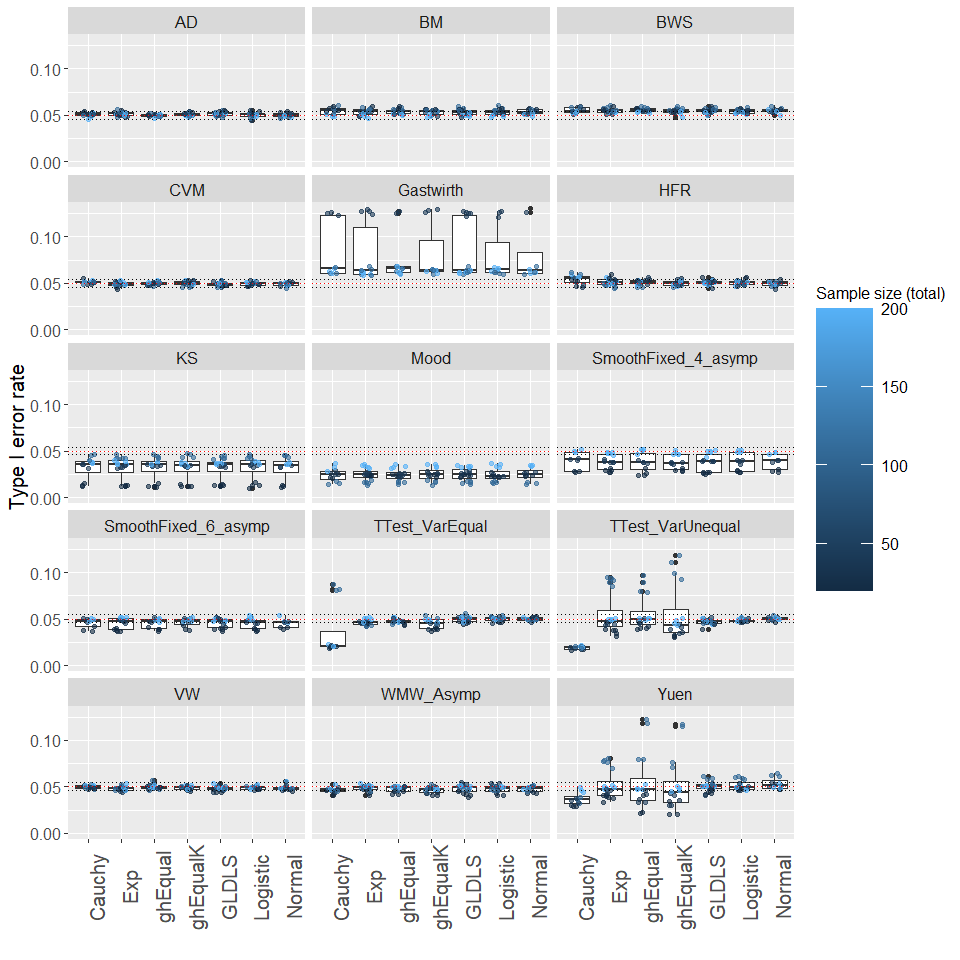
\includegraphics{report_files/figure-latex/unnamed-chunk-2-1.pdf}

\hypertarget{power-power-curve-best-method}{%
\subsection{3. Power-power curve: Best
method}\label{power-power-curve-best-method}}

In the figures below (Figure:2-5), the power-power curves are shown
between the specified method versus the `best' performing method in that
specific scenario setting (distribution). These plots are given for
sample size 20 (left column) and sample size 200 (right column). All 14
methods are included, we excluded Gastwirth as the method had a type I
error rate that was far too liberal for most scenarios. In general, the
results with sample size 20 are more scattered, while the results of
sample size 200 are more centered around the diagonal and more
specifically the top right of the diagonal (highest power results),
which is expected as the power increases with sample size. The tests
that had a very conservative type I error rate control (KS, Mood), also
show power-power curves that reflect the lack of power in comparison to
the best performing methods. This lack in power is also noticeable for
the results for the Cauchy and g-h distributions of the two sample
Student-t test and the Welch t-test. Remarkably, for some scenarios of
the normal distributions with unequal variances, the Welch t-test has
much lower power than the best competitor, the best competitor is the
two sample smooth test with fixed order 4 and Legendre polynomials. For
the WMW test, the power-power plot shows that the test has at least
similar results in comparison to the best method for the logistic
distribution with sample size 200 (as expected), but for the small
sample sizes slightly better tests exist. The plots of
Anderson-Darling(AD) have more of the observations around the diagonal
for both sample sizes in comparison to all other methods. Hence, the AD
test has often the largest power, and when it does not, its power is not
much smaller than the power of the best competitor (i.e.~the points are
close to the diagonal). The worst performing test is the two sample
smooth test with fixed order 6 and Legendre Polynomials. Based on these
results we selected AD, KS, the Welsh test, Student-t test, WmW test and
two sample smooth test with fixed order 4 and Legendre polynomials.
Hence, the plots are better evaluated in some more detail in the next
section.

\textbackslash begin\{figure\}{[}H{]}
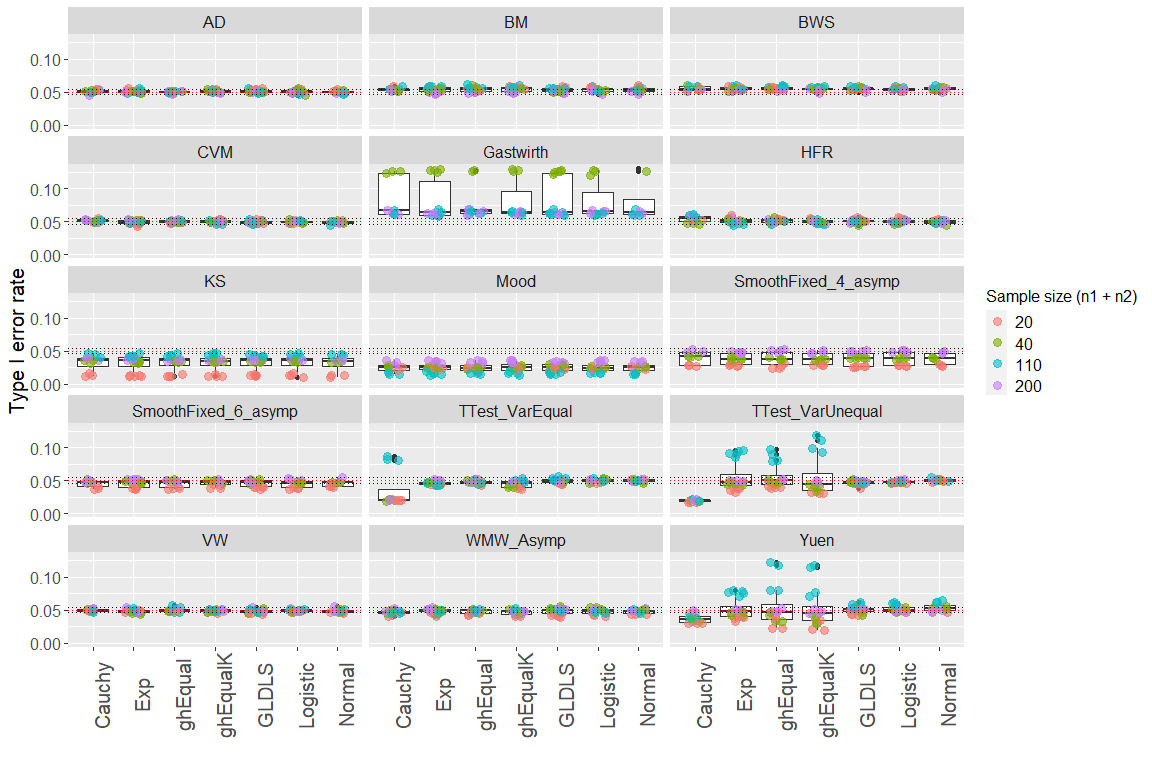
\includegraphics[width=0.5\linewidth]{report_files/figure-latex/unnamed-chunk-4-1}
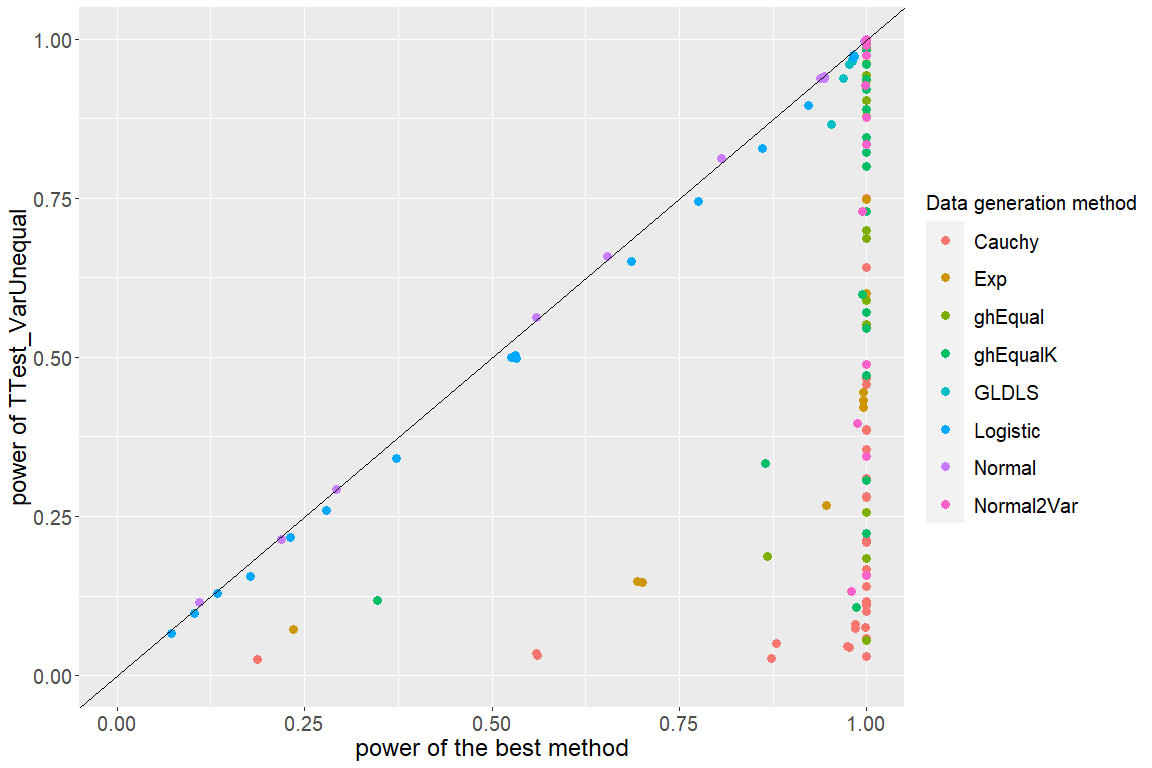
\includegraphics[width=0.5\linewidth]{report_files/figure-latex/unnamed-chunk-4-2}
\textbackslash caption\{Left:(n=20) AD has the largest power in 52 of
the 176 scenarios, which is 29.55 \% of the scenarios. The median of the
power differences for scenarios where AD has smaller power than the best
test is 0.0316 --- Right: (n=200) AD has the largest power in 1 of the
225 scenarios, which is 0.44 \% of the scenarios. The median of the
power differences for scenarios where AD has smaller power than the best
test is 0.0094\}\label{fig:unnamed-chunk-4} \textbackslash end\{figure\}

\textbackslash begin\{figure\}{[}H{]}
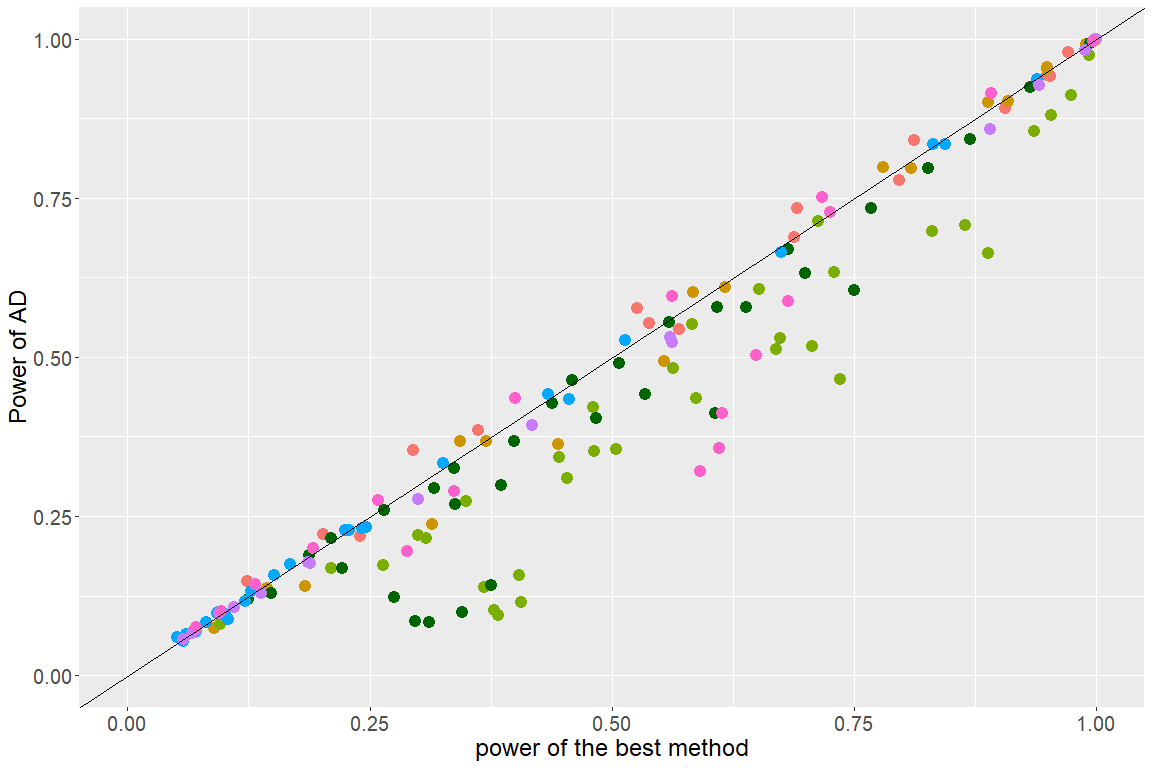
\includegraphics[width=0.5\linewidth]{report_files/figure-latex/unnamed-chunk-6-1}
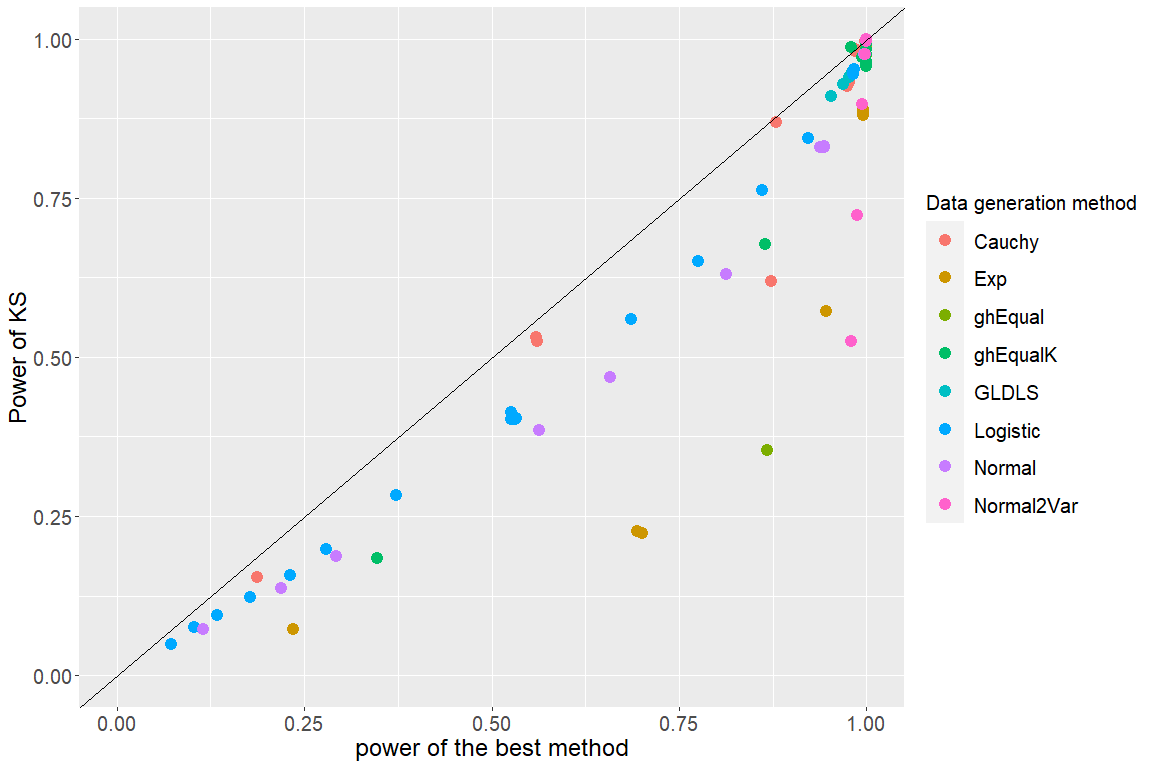
\includegraphics[width=0.5\linewidth]{report_files/figure-latex/unnamed-chunk-6-2}
\textbackslash caption\{Left:(n=20) KS has the largest power in 0 of the
225 scenarios, which is 0 \% of the scenarios. The median of the power
differences for scenarios where KS has smaller power than the best test
is 0.1635 --- Right: (n=200) KS has the largest power in 1 of the 225
scenarios, which is 0.44 \% of the scenarios. The median of the power
differences for scenarios where KS has smaller power than the best test
is 0.0357\}\label{fig:unnamed-chunk-6} \textbackslash end\{figure\}

\textbackslash begin\{figure\}{[}H{]}
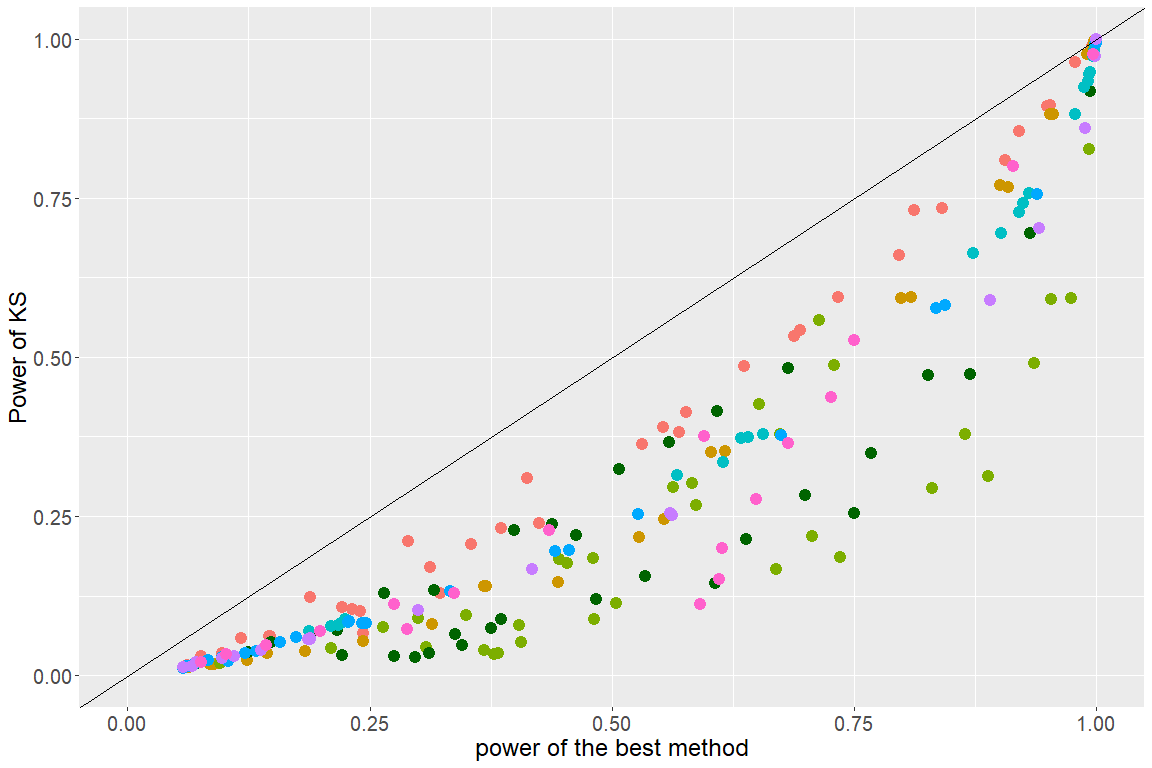
\includegraphics[width=0.5\linewidth]{report_files/figure-latex/unnamed-chunk-8-1}
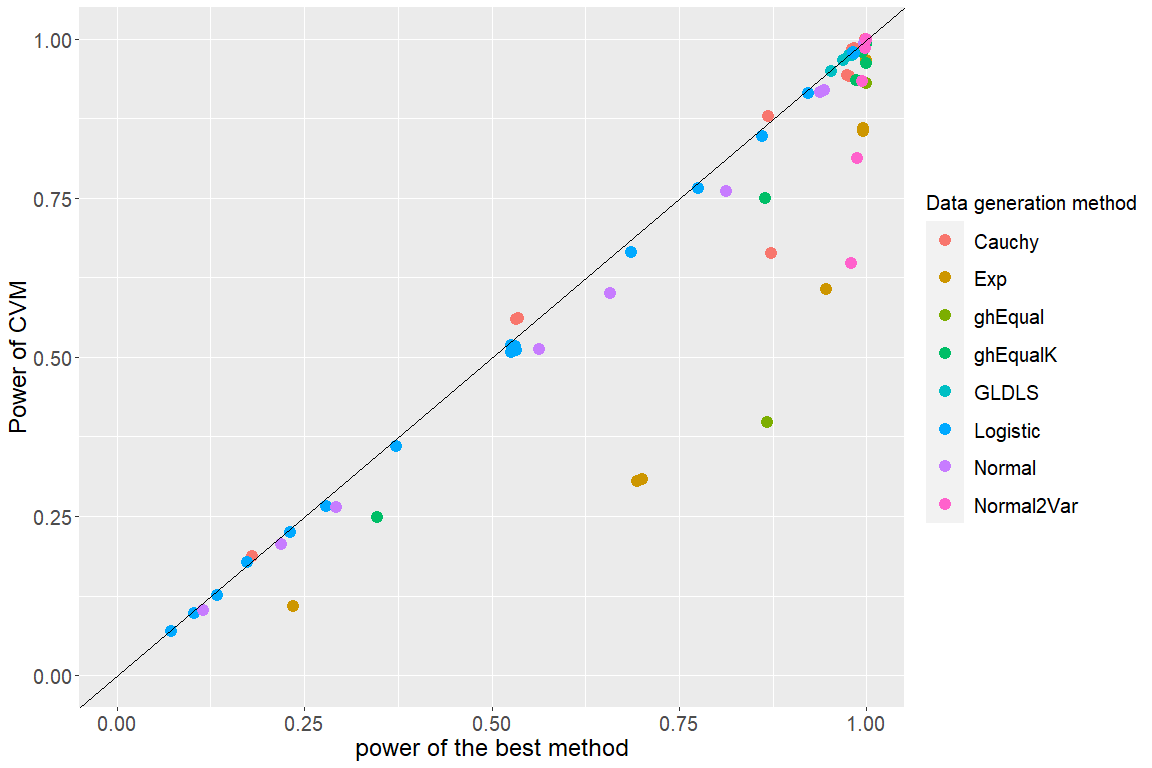
\includegraphics[width=0.5\linewidth]{report_files/figure-latex/unnamed-chunk-8-2}
\textbackslash caption\{Left:(n=20) CVM has the largest power in 32 of
the 207 scenarios, which is 15.46 \% of the scenarios. The median of the
power differences for scenarios where CVM has smaller power than the
best test is 0.0291 --- Right: (n=200) CVM has the largest power in 9 of
the 225 scenarios, which is 4 \% of the scenarios. The median of the
power differences for scenarios where CVM has smaller power than the
best test is 0.0078\}\label{fig:unnamed-chunk-8}
\textbackslash end\{figure\}

\textbackslash begin\{figure\}{[}H{]}
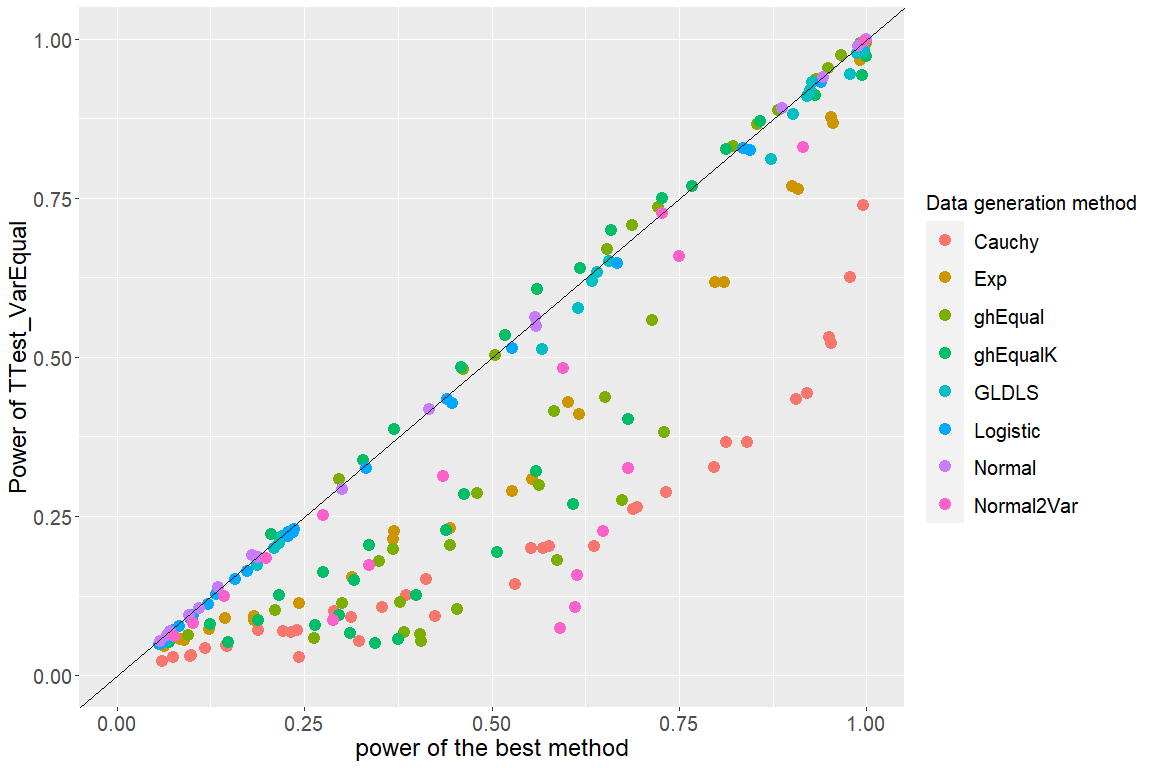
\includegraphics[width=0.5\linewidth]{report_files/figure-latex/unnamed-chunk-10-1}
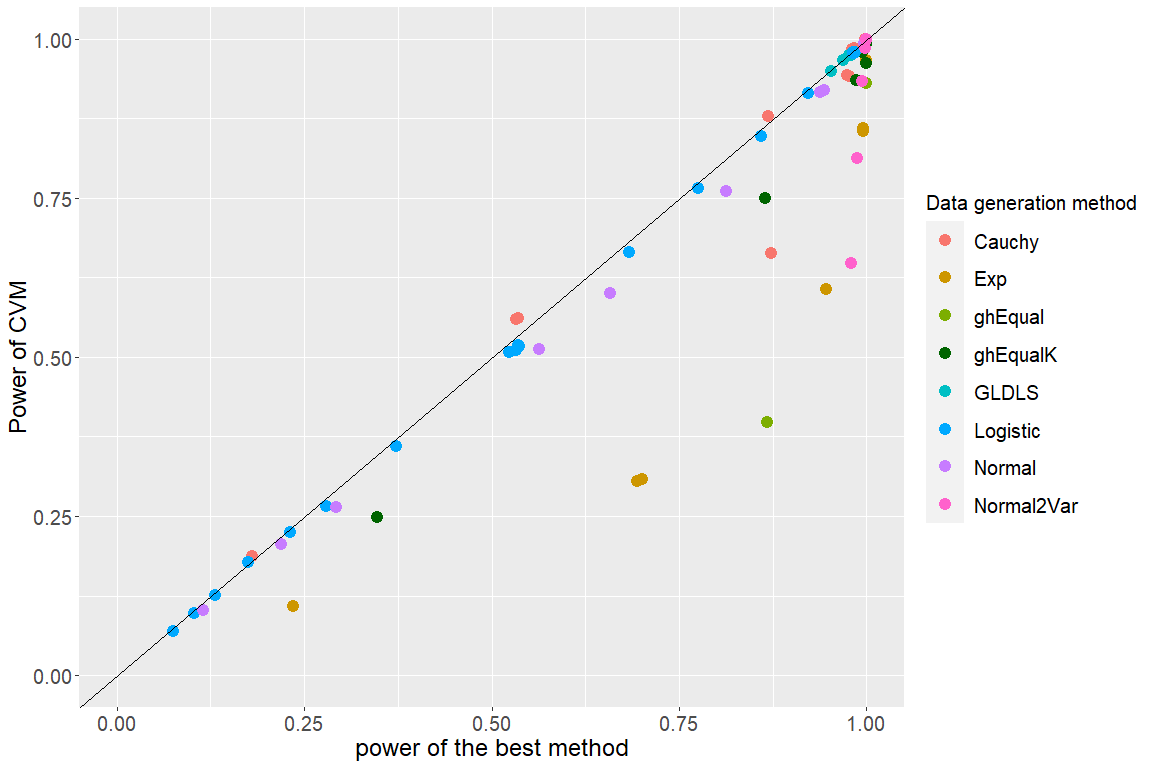
\includegraphics[width=0.5\linewidth]{report_files/figure-latex/unnamed-chunk-10-2}
\textbackslash caption\{Left:(n=20) TTest\_VarEqual has the largest
power in 31 of the 225 scenarios, which is 13.78 \% of the scenarios.
The median of the power differences for scenarios where TTest\_VarEqual
has smaller power than the best test is 0.0866 --- Right: (n=200)
TTest\_VarEqual has the largest power in 5 of the 225 scenarios, which
is 2.22 \% of the scenarios. The median of the power differences for
scenarios where TTest\_VarEqual has smaller power than the best test is
0.162\}\label{fig:unnamed-chunk-10} \textbackslash end\{figure\}

\textbackslash begin\{figure\}{[}H{]}
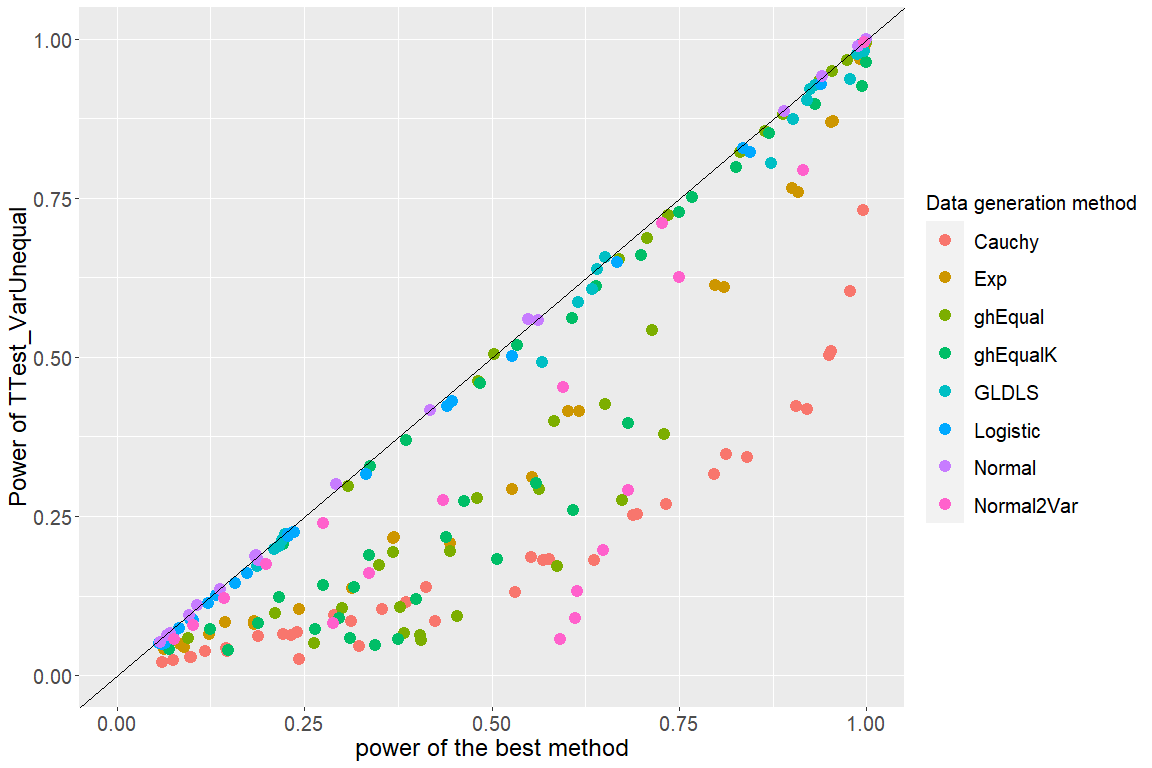
\includegraphics[width=0.5\linewidth]{report_files/figure-latex/unnamed-chunk-12-1}
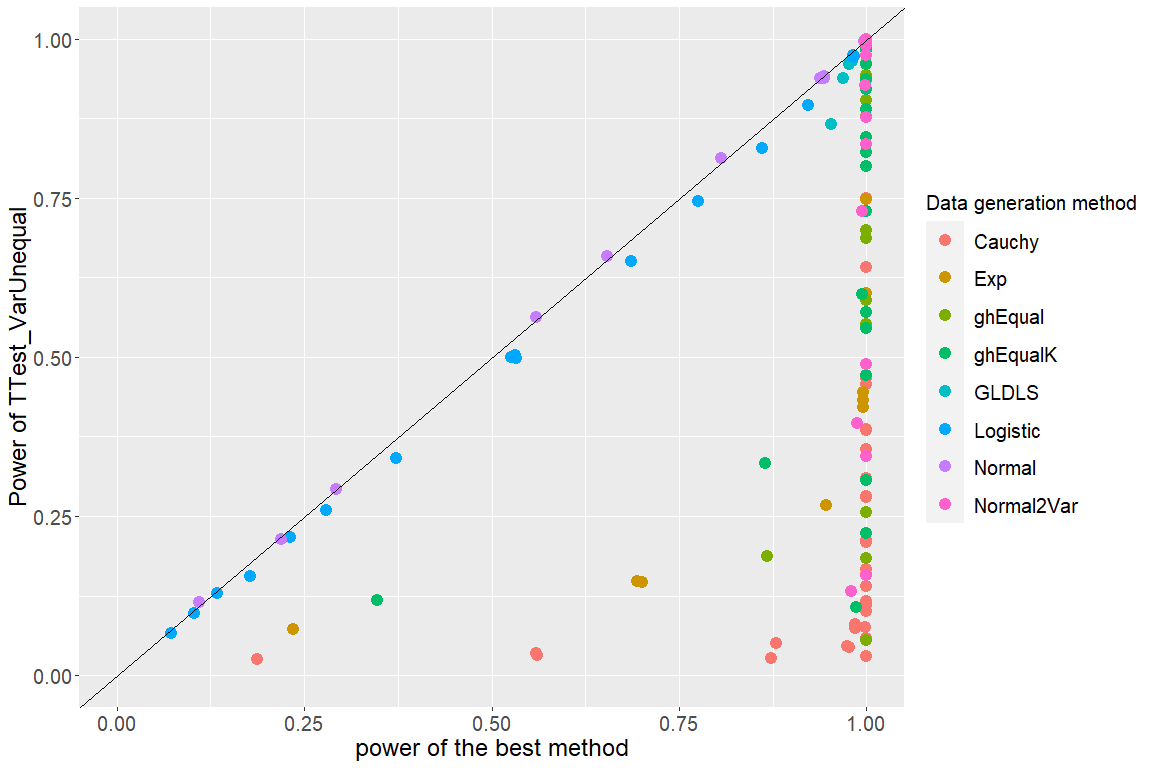
\includegraphics[width=0.5\linewidth]{report_files/figure-latex/unnamed-chunk-12-2}
\textbackslash caption\{Left:(n=20) TTest\_VarUnequal has the largest
power in 8 of the 225 scenarios, which is 3.56 \% of the scenarios. The
median of the power differences for scenarios where TTest\_VarUnequal
has smaller power than the best test is 0.0455 --- Right: (n=200)
TTest\_VarUnequal has the largest power in 5 of the 225 scenarios, which
is 2.22 \% of the scenarios. The median of the power differences for
scenarios where TTest\_VarUnequal has smaller power than the best test
is 0.1622\}\label{fig:unnamed-chunk-12} \textbackslash end\{figure\}

\textbackslash begin\{figure\}{[}H{]}
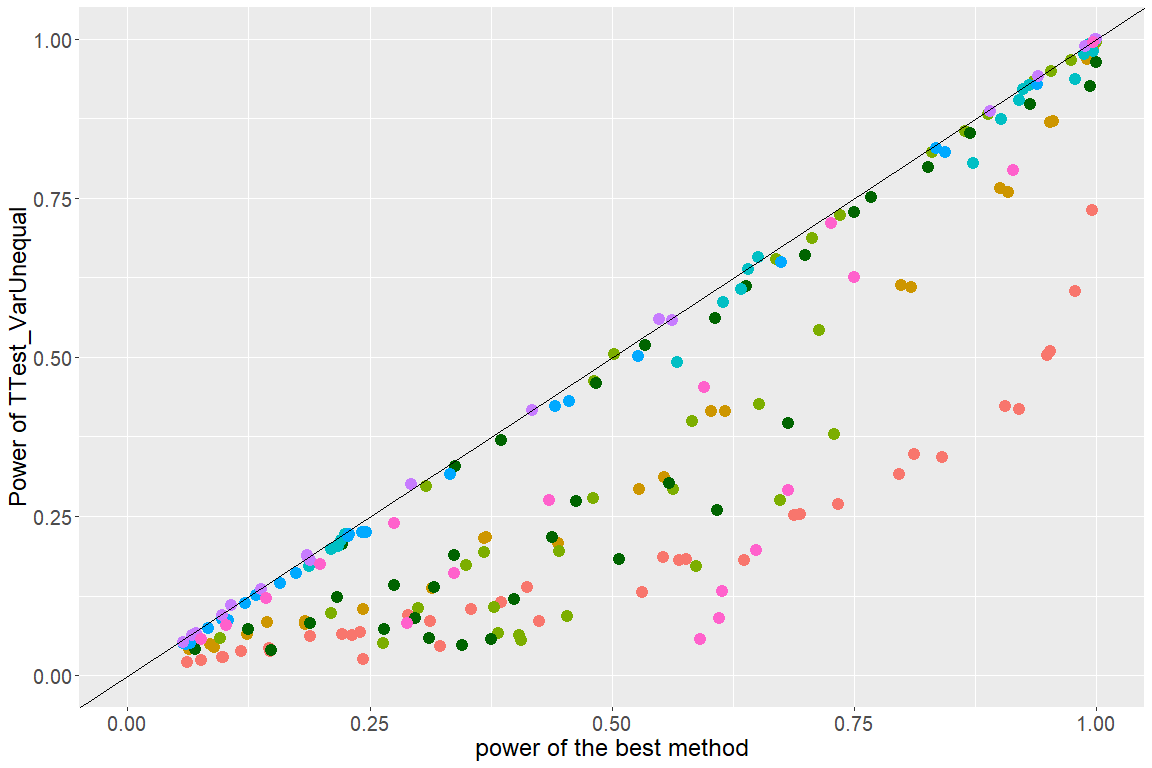
\includegraphics[width=0.5\linewidth]{report_files/figure-latex/unnamed-chunk-14-1}
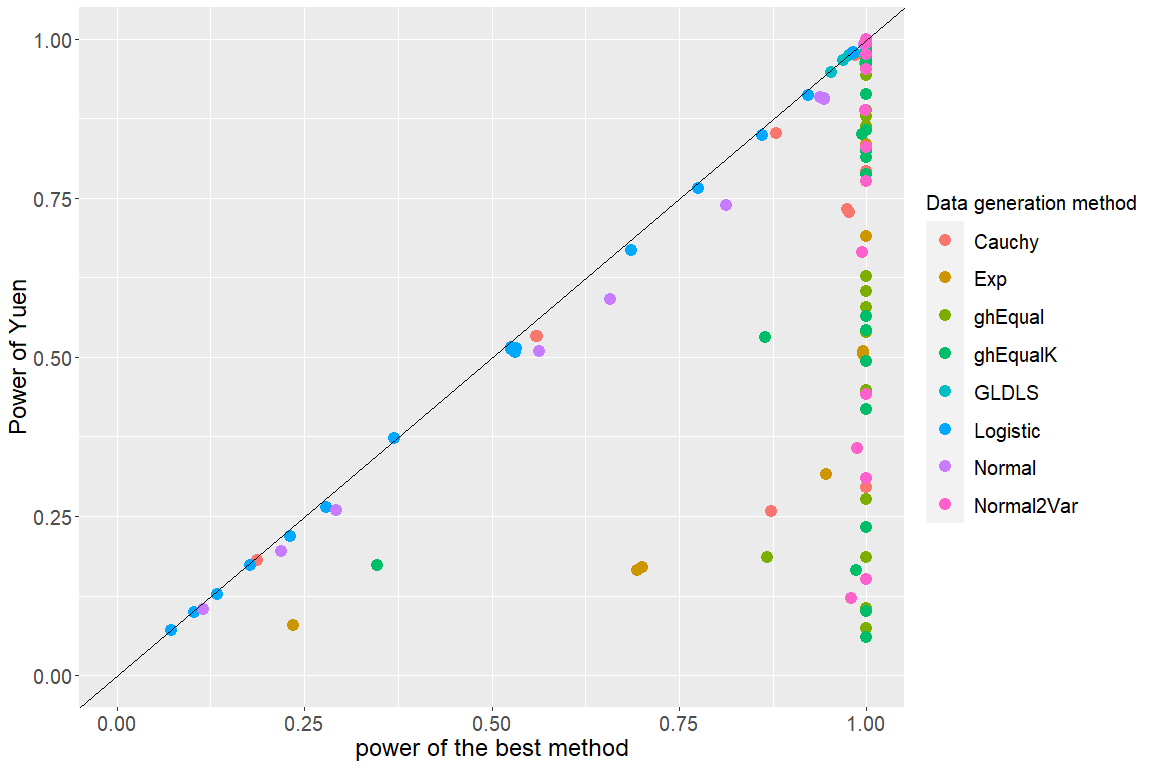
\includegraphics[width=0.5\linewidth]{report_files/figure-latex/unnamed-chunk-14-2}
\textbackslash caption\{Left:(n=20) Yuen has the largest power in 7 of
the 225 scenarios, which is 3.11 \% of the scenarios. The median of the
power differences for scenarios where Yuen has smaller power than the
best test is 0.0758 --- Right: (n=200) Yuen has the largest power in 1
of the 225 scenarios, which is 0.44 \% of the scenarios. The median of
the power differences for scenarios where Yuen has smaller power than
the best test is 0.029\}\label{fig:unnamed-chunk-14}
\textbackslash end\{figure\}

\textbackslash begin\{figure\}{[}H{]}
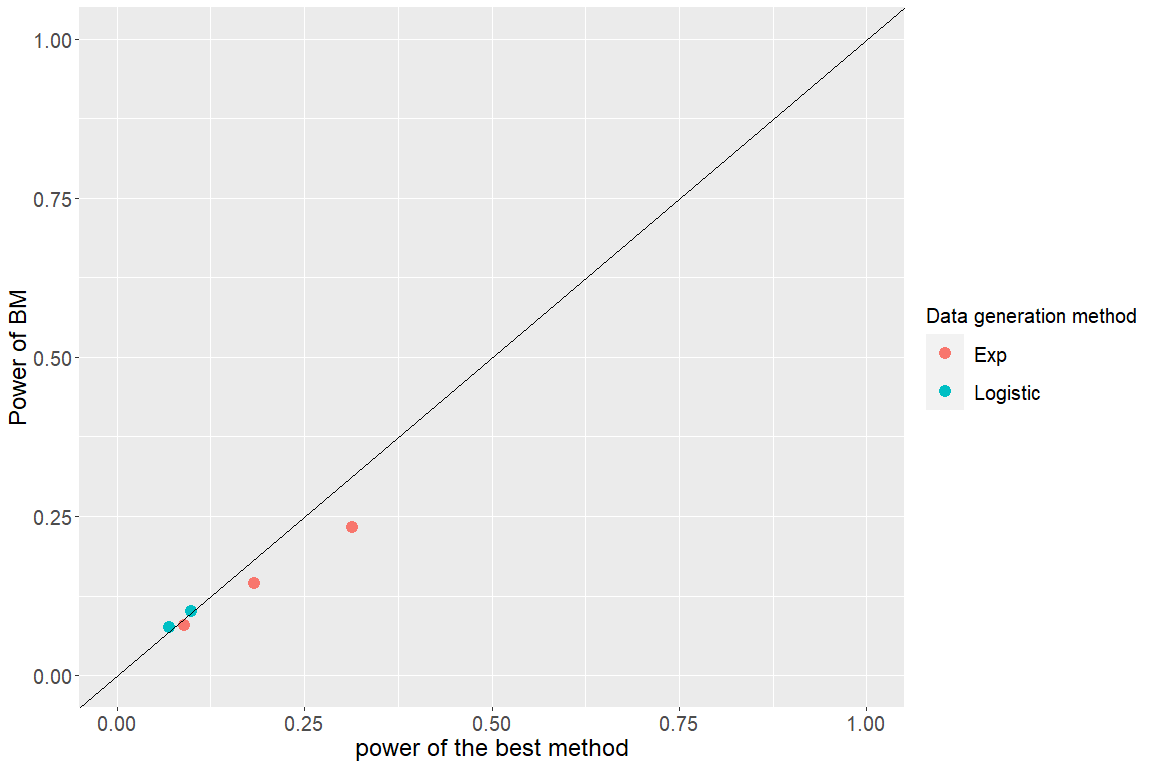
\includegraphics[width=0.5\linewidth]{report_files/figure-latex/unnamed-chunk-16-1}
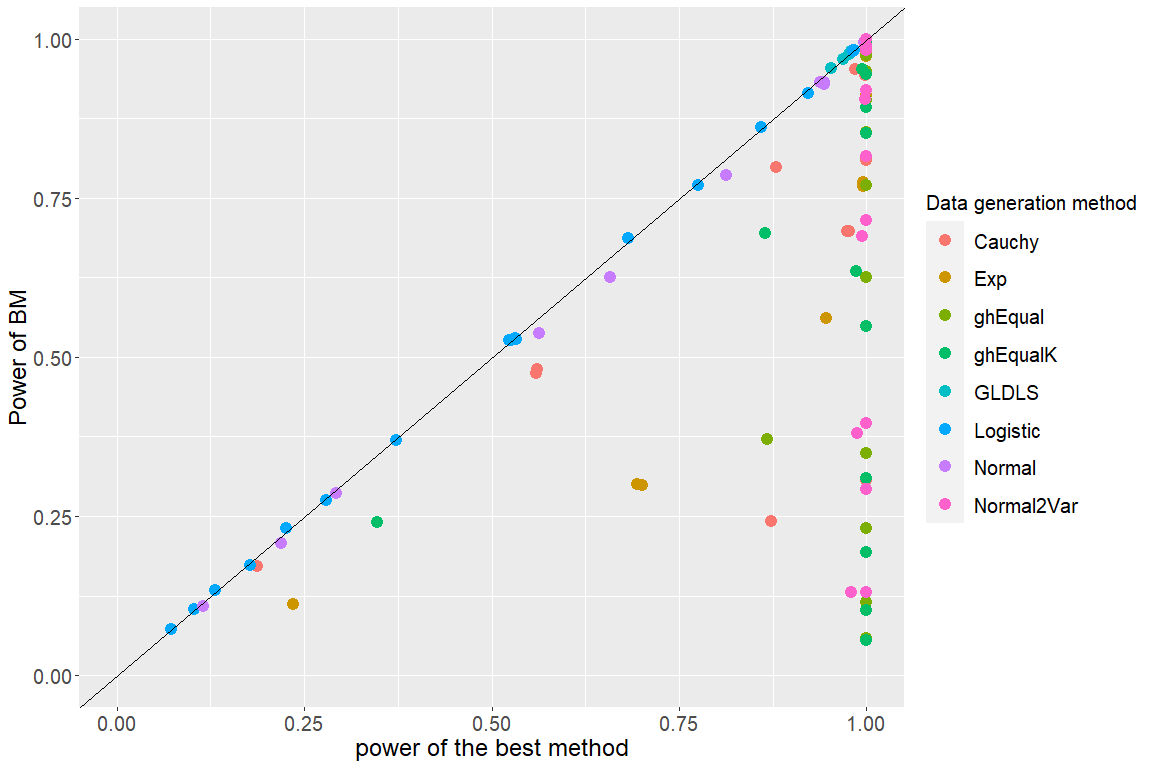
\includegraphics[width=0.5\linewidth]{report_files/figure-latex/unnamed-chunk-16-2}
\textbackslash caption\{Left:(n=20) BM has the largest power in 2 of the
5 scenarios, which is 40 \% of the scenarios. The median of the power
differences for scenarios where BM has smaller power than the best test
is 0.0387 --- Right: (n=200) BM has the largest power in 8 of the 212
scenarios, which is 3.77 \% of the scenarios. The median of the power
differences for scenarios where BM has smaller power than the best test
is 0.0179\}\label{fig:unnamed-chunk-16} \textbackslash end\{figure\}

\textbackslash begin\{figure\}{[}H{]}
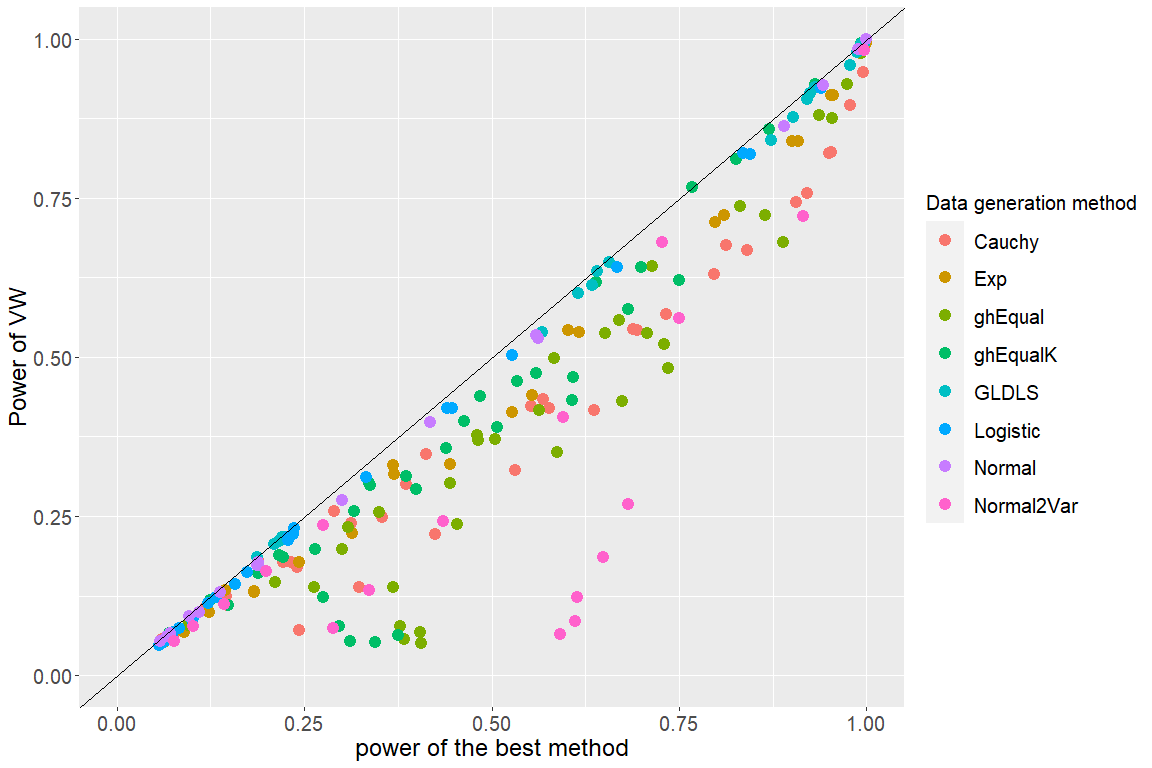
\includegraphics[width=0.5\linewidth]{report_files/figure-latex/unnamed-chunk-18-1}
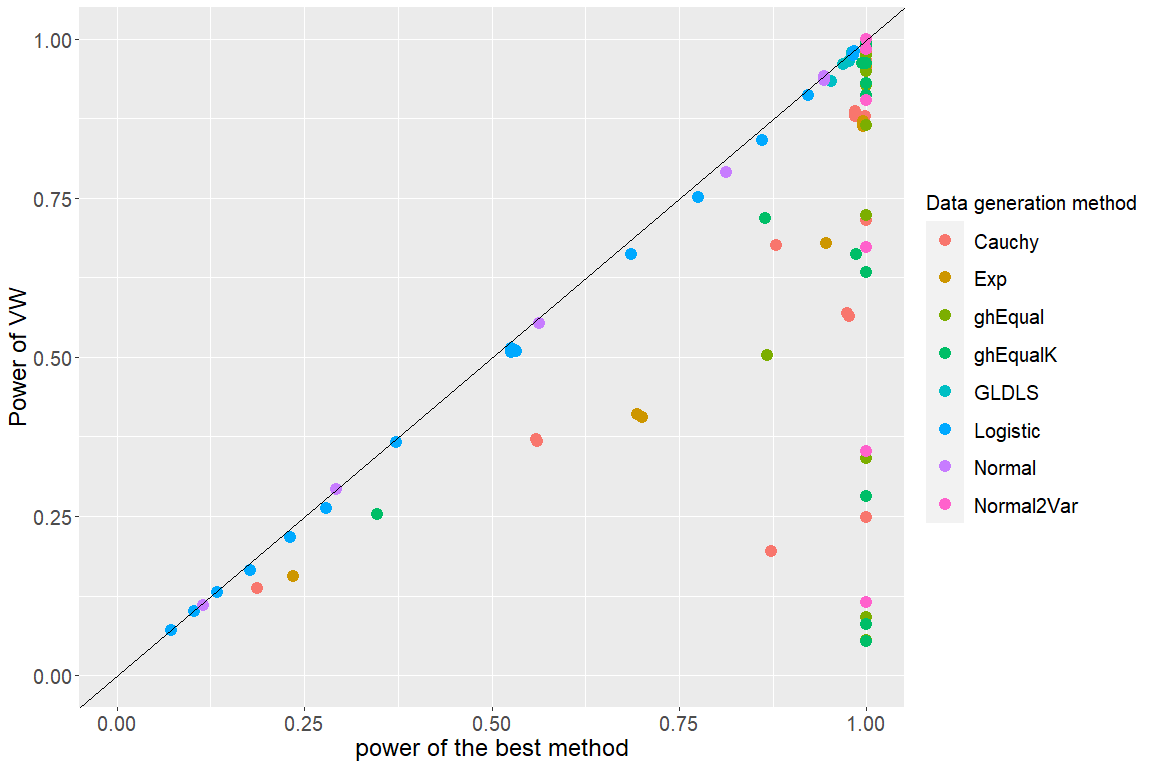
\includegraphics[width=0.5\linewidth]{report_files/figure-latex/unnamed-chunk-18-2}
\textbackslash caption\{Left:(n=20) VW has the largest power in 1 of the
225 scenarios, which is 0.44 \% of the scenarios. The median of the
power differences for scenarios where VW has smaller power than the best
test is 0.0377 --- Right: (n=200) VW has the largest power in 0 of the
207 scenarios, which is 0 \% of the scenarios. The median of the power
differences for scenarios where VW has smaller power than the best test
is 0.02\}\label{fig:unnamed-chunk-18} \textbackslash end\{figure\}

\textbackslash begin\{figure\}{[}H{]}
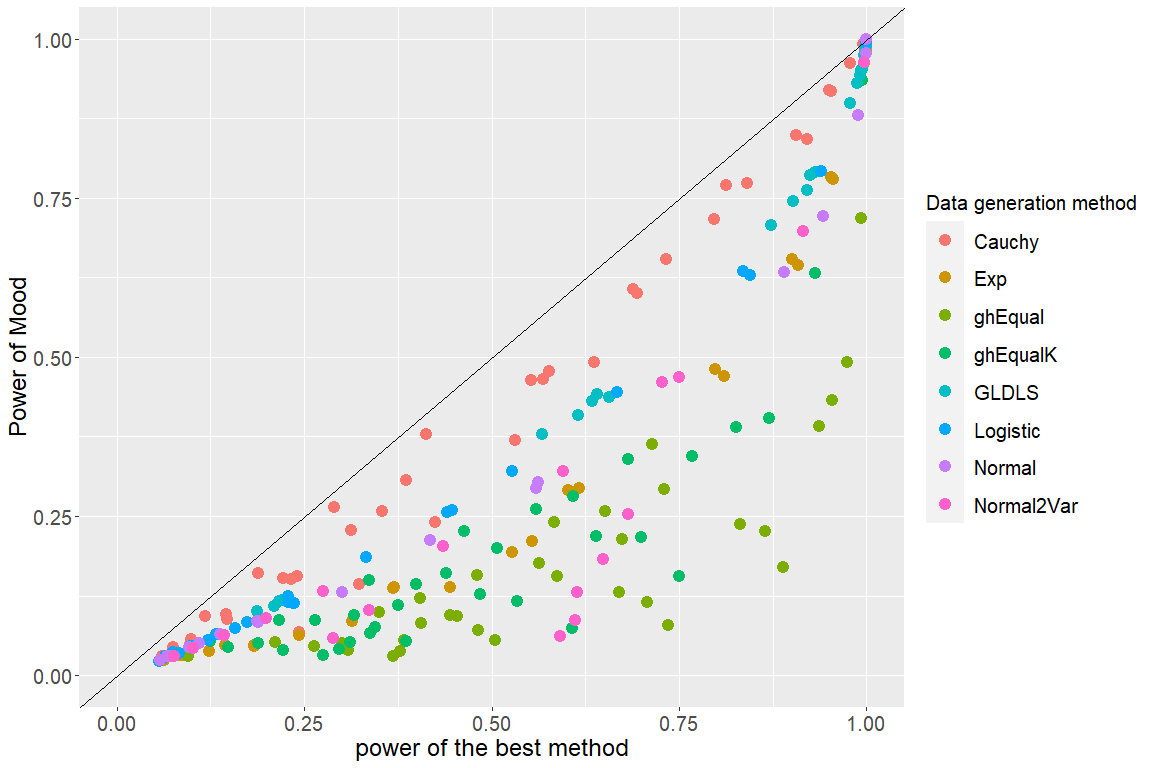
\includegraphics[width=0.5\linewidth]{report_files/figure-latex/unnamed-chunk-20-1}
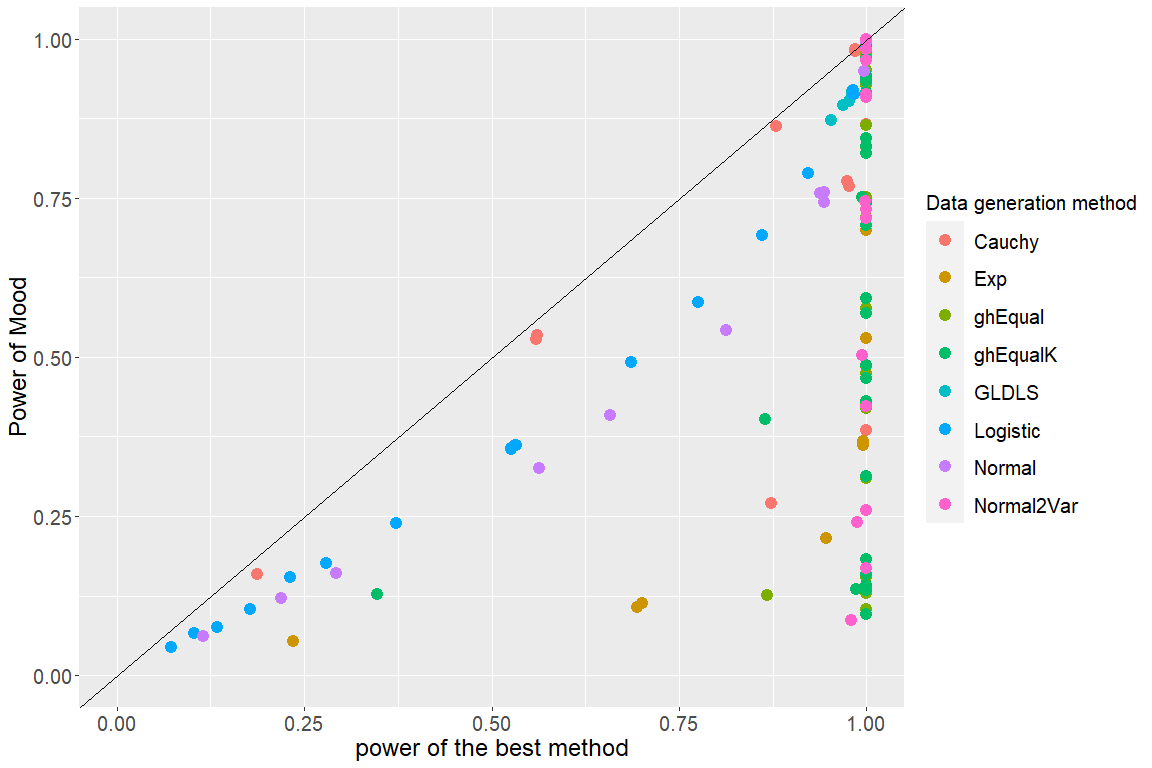
\includegraphics[width=0.5\linewidth]{report_files/figure-latex/unnamed-chunk-20-2}
\textbackslash caption\{Left:(n=20) Mood has the largest power in 0 of
the 225 scenarios, which is 0 \% of the scenarios. The median of the
power differences for scenarios where Mood has smaller power than the
best test is 0.1575 --- Right: (n=200) Mood has the largest power in 0
of the 225 scenarios, which is 0 \% of the scenarios. The median of the
power differences for scenarios where Mood has smaller power than the
best test is 0.1337\}\label{fig:unnamed-chunk-20}
\textbackslash end\{figure\}

\textbackslash begin\{figure\}{[}H{]}
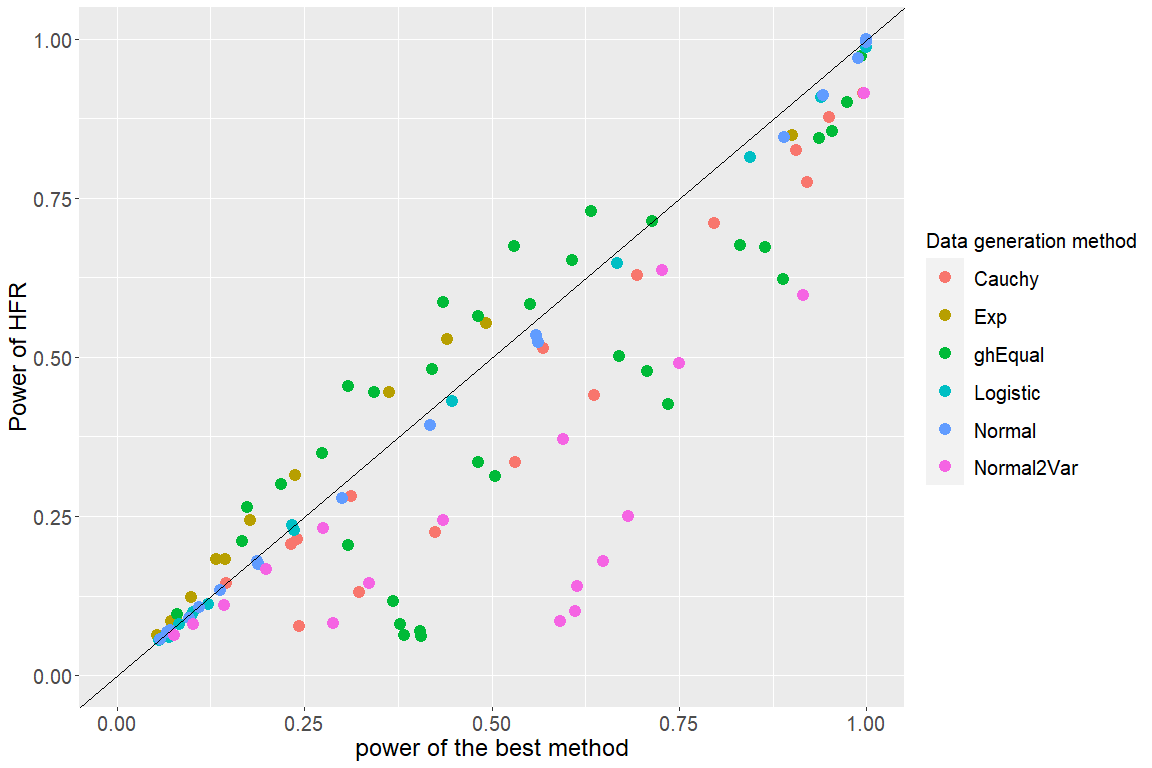
\includegraphics[width=0.5\linewidth]{report_files/figure-latex/unnamed-chunk-22-1}
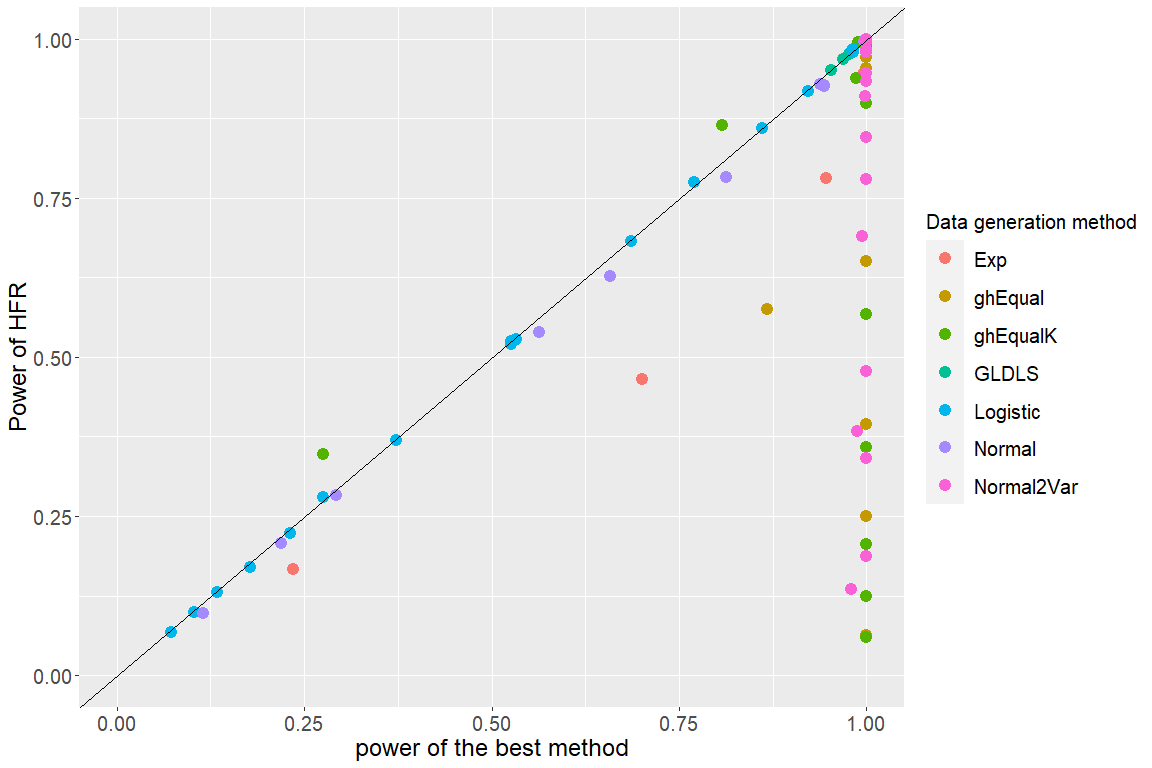
\includegraphics[width=0.5\linewidth]{report_files/figure-latex/unnamed-chunk-22-2}
\textbackslash caption\{Left:(n=20) HFR has the largest power in 28 of
the 115 scenarios, which is 24.35 \% of the scenarios. The median of the
power differences for scenarios where HFR has smaller power than the
best test is 0.0523 --- Right: (n=200) HFR has the largest power in 8 of
the 183 scenarios, which is 4.37 \% of the scenarios. The median of the
power differences for scenarios where HFR has smaller power than the
best test is 0.0116\}\label{fig:unnamed-chunk-22}
\textbackslash end\{figure\}

\textbackslash begin\{figure\}{[}H{]}
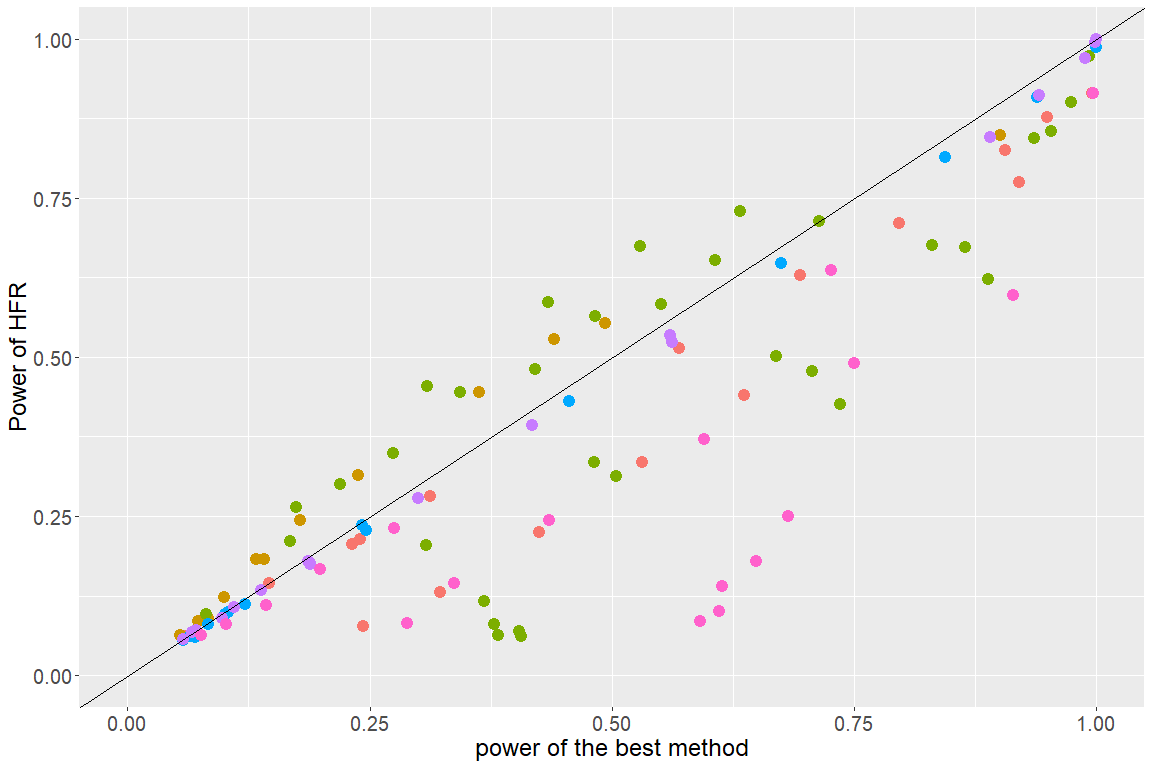
\includegraphics[width=0.5\linewidth]{report_files/figure-latex/unnamed-chunk-24-1}
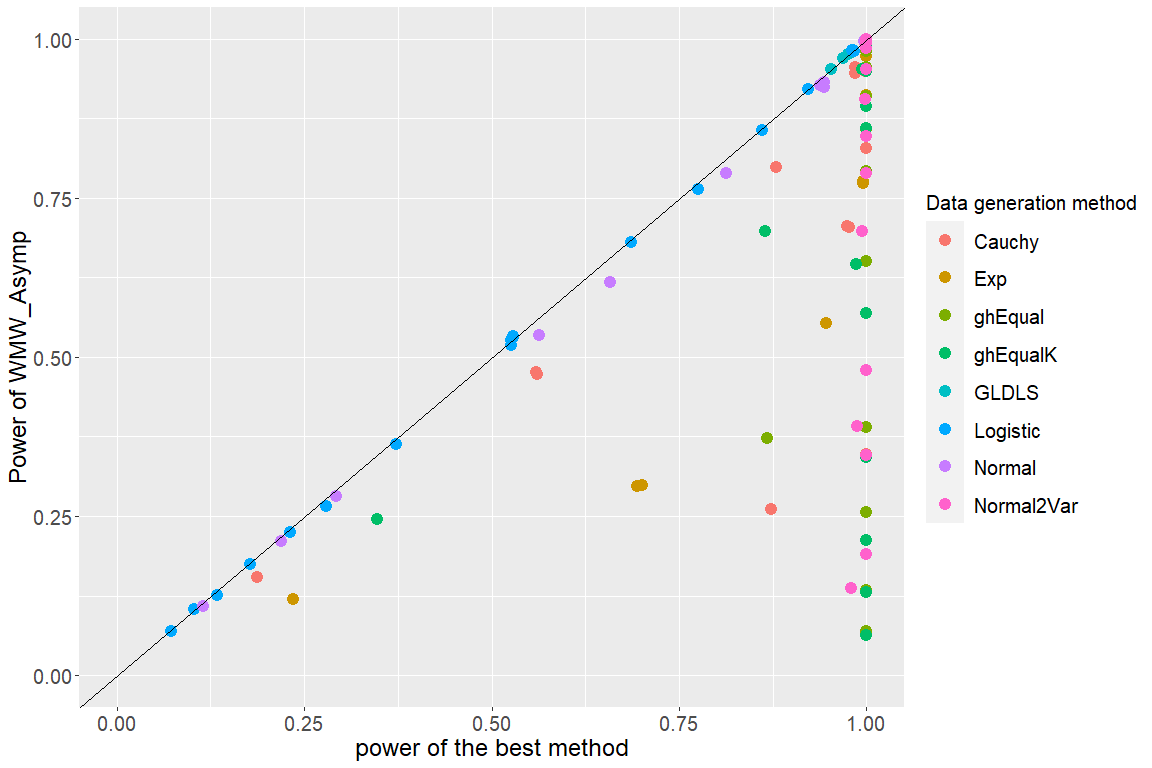
\includegraphics[width=0.5\linewidth]{report_files/figure-latex/unnamed-chunk-24-2}
\textbackslash caption\{Left:(n=20) WMW\_Asymp has the largest power in
1 of the 225 scenarios, which is 0.44 \% of the scenarios. The median of
the power differences for scenarios where WMW\_Asymp has smaller power
than the best test is 0.0478 --- Right: (n=200) WMW\_Asymp has the
largest power in 8 of the 225 scenarios, which is 3.56 \% of the
scenarios. The median of the power differences for scenarios where
WMW\_Asymp has smaller power than the best test is
0.0193\}\label{fig:unnamed-chunk-24} \textbackslash end\{figure\}

\textbackslash begin\{figure\}{[}H{]}
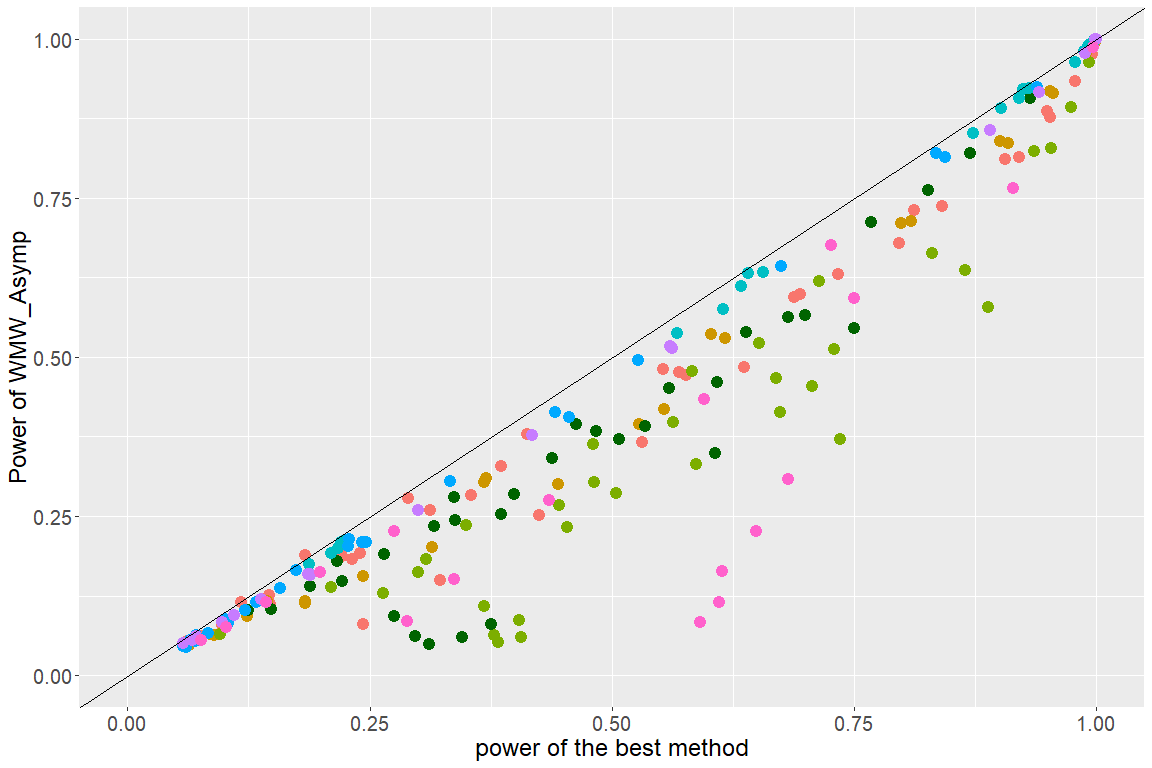
\includegraphics[width=0.5\linewidth]{report_files/figure-latex/unnamed-chunk-26-1}
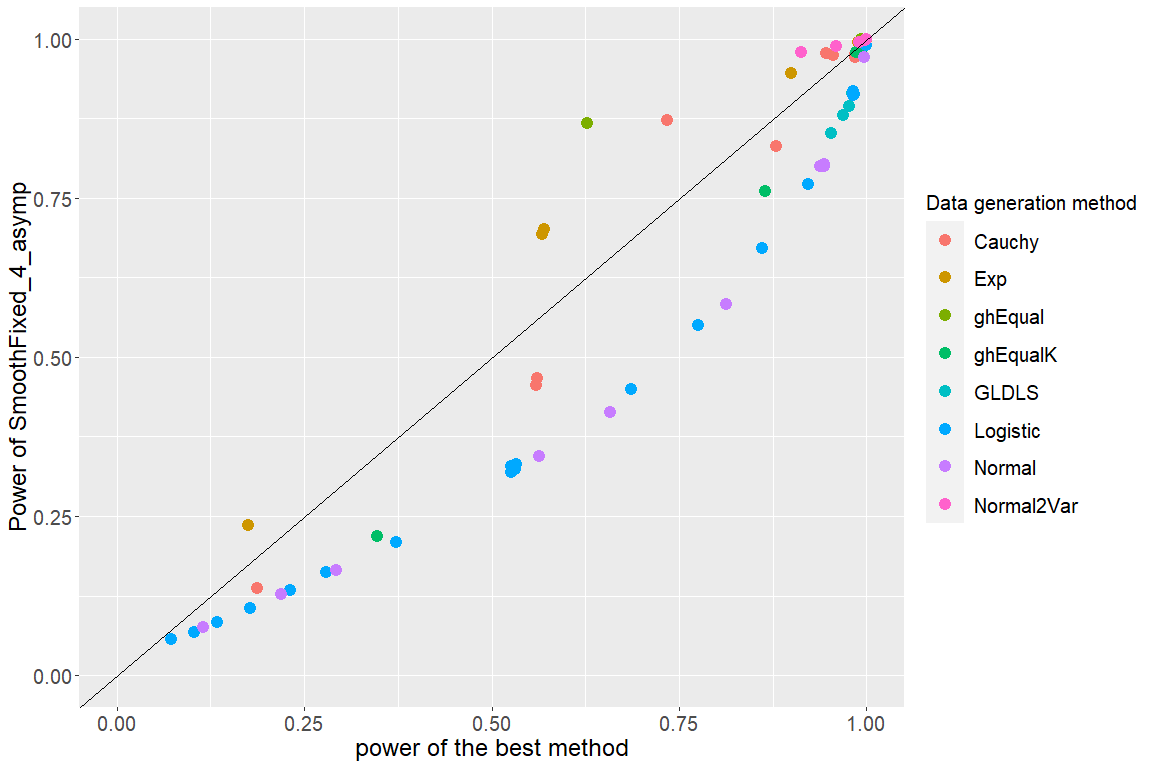
\includegraphics[width=0.5\linewidth]{report_files/figure-latex/unnamed-chunk-26-2}
\textbackslash caption\{Left:(n=20) SmoothFixed\_4\_asymp has the
largest power in 24 of the 225 scenarios, which is 10.67 \% of the
scenarios. The median of the power differences for scenarios where
SmoothFixed\_4\_asymp has smaller power than the best test is 0.132 ---
Right: (n=200) SmoothFixed\_4\_asymp has the largest power in 23 of the
225 scenarios, which is 10.22 \% of the scenarios. The median of the
power differences for scenarios where SmoothFixed\_4\_asymp has smaller
power than the best test is 0.071\}\label{fig:unnamed-chunk-26}
\textbackslash end\{figure\}

\textbackslash begin\{figure\}{[}H{]}
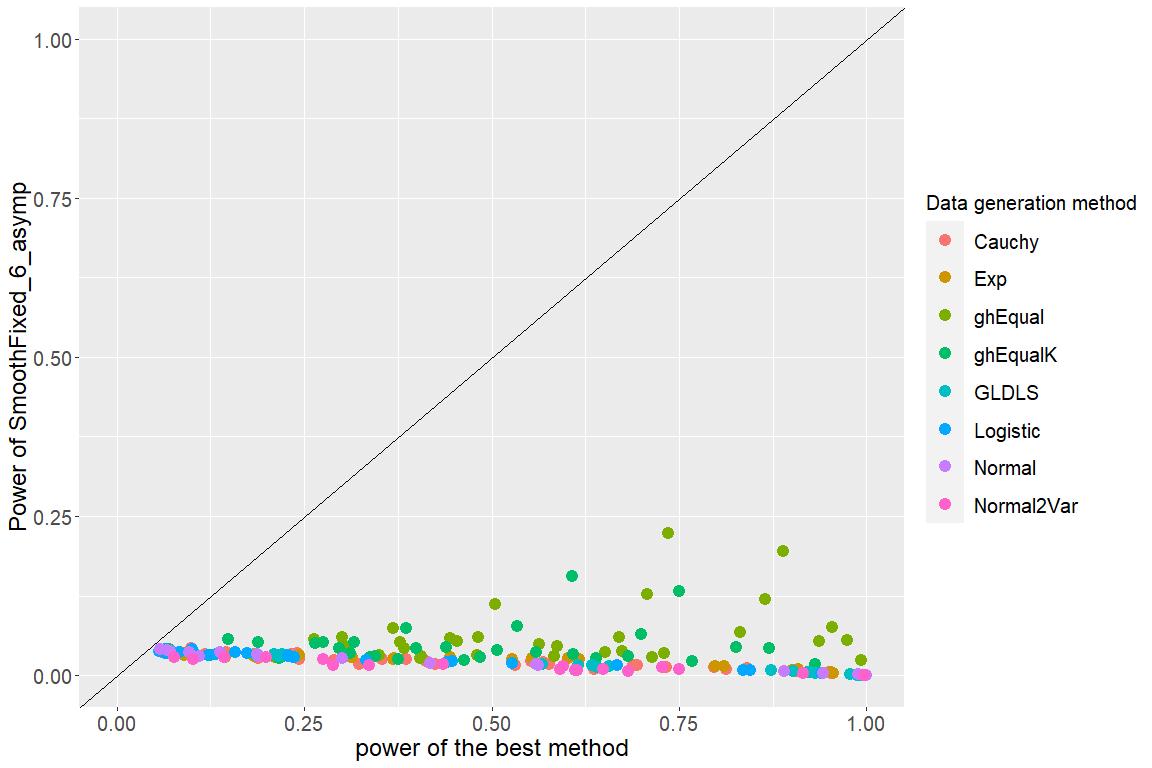
\includegraphics[width=0.5\linewidth]{report_files/figure-latex/unnamed-chunk-28-1}
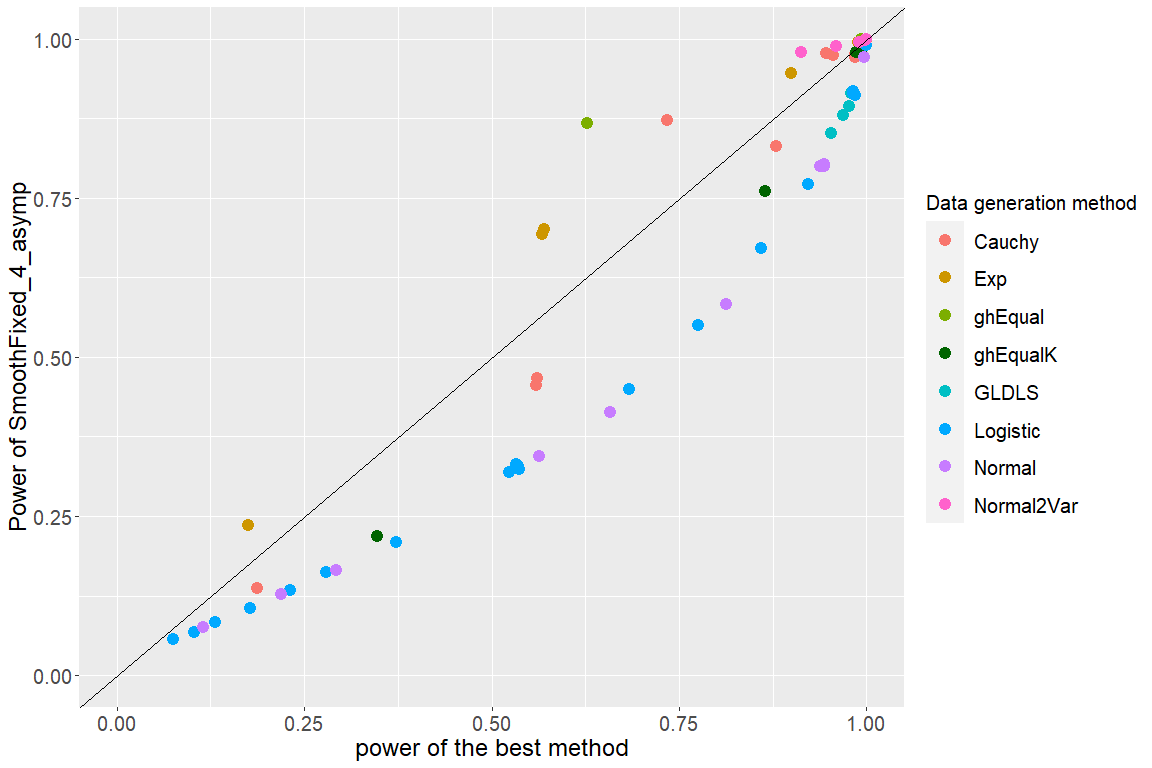
\includegraphics[width=0.5\linewidth]{report_files/figure-latex/unnamed-chunk-28-2}
\textbackslash caption\{Left:(n=20) SmoothFixed\_6\_asymp has the
largest power in 0 of the 225 scenarios, which is 0 \% of the scenarios.
The median of the power differences for scenarios where
SmoothFixed\_6\_asymp has smaller power than the best test is 0.4511 ---
Right: (n=200) SmoothFixed\_6\_asymp has the largest power in 0 of the
225 scenarios, which is 0 \% of the scenarios. The median of the power
differences for scenarios where SmoothFixed\_6\_asymp has smaller power
than the best test is 0.8241\}\label{fig:unnamed-chunk-28}
\textbackslash end\{figure\}

\hypertarget{power-power-curve}{%
\subsection{4. Power-Power curve}\label{power-power-curve}}

The power-power plots are based on 10000 simulation runs and 5\%
significance level. The scenarios where the type I error was too liberal
are filtered out. The first comparison (Figure 3, top left), the
Anderson-Darling test (AD) versus the Kolmogrov Smirnov test (KS), shows
that AD has a higher power in most scenarios. For some scenario's in the
Cauchy distribution and Normal distribution with unequal variances, KS
has a higher power. These scenarios are characterized with unequal
sample sizes. Moreover, the asymmetry of the plot suggests that when the
AD outperforms the KS test, it is by a larger margin than it is the
other way around. The power-power plot of the two sample student t-test
and the Welch test (Figure 6, top right), show the results of most
scenarios are close to the diagonal which means that they have similar
results in those scenarios. However for the scenarios from the Normal
distribution with unequal variances and unequal sample sizes, the Welch
test outperforms the two sample student-t test. The third comparison
(Figure 6, down left), compares the Welch t-test to the
Wilcoxon-Mann-Whitney test (WMW). In this comparison it's clear that WMW
outperforms the Welch t-test for scenarios from the Cauchy and
Exponential distribution. The plot also shows that many points are close
to the diagonal (particularly for the symmetric distributions),
indicating that for these distributions the powers of the two tests are
close to one another. However, there are still many other points far off
the diagonal, towards both sides. This shows that for some scenarios
(skew and/or heavy tailed distributions) the powers of the WMW test and
the Welch t-test may be very different. Sometimes the WMW wins, other
times the Welch t-test wins. The last plot (Figure 6, down right)
compares WMW with Two sample smooth test with fixed order 4 and Legendre
polynomials. WMW outperforms the smooth test in the logistic
distribution, and has a higher power in the scenarios that come from the
more symmetric distributions. In contrast, the smooth test has a higher
power in the more skewed and/or heavy tailed distributions, which is
what we would expect from the smooth test.

\begin{figure}[H]
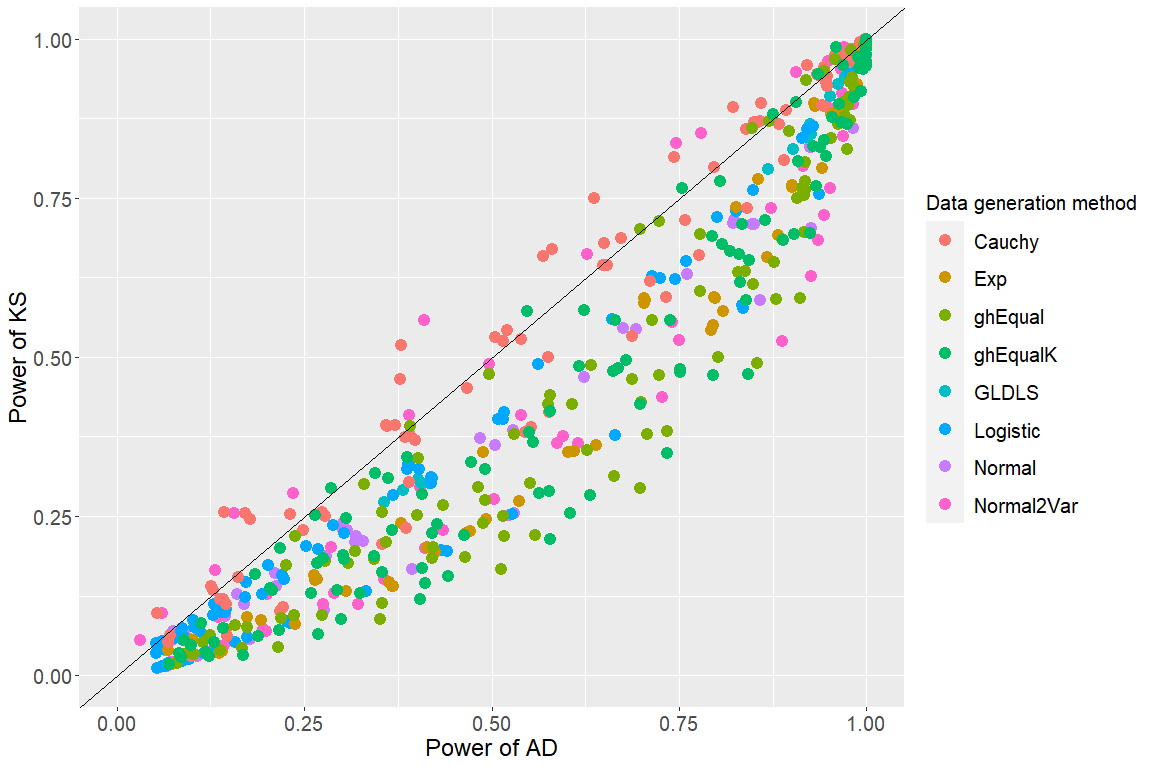
\includegraphics[width=0.5\linewidth]{report_files/figure-latex/figures-side-1} 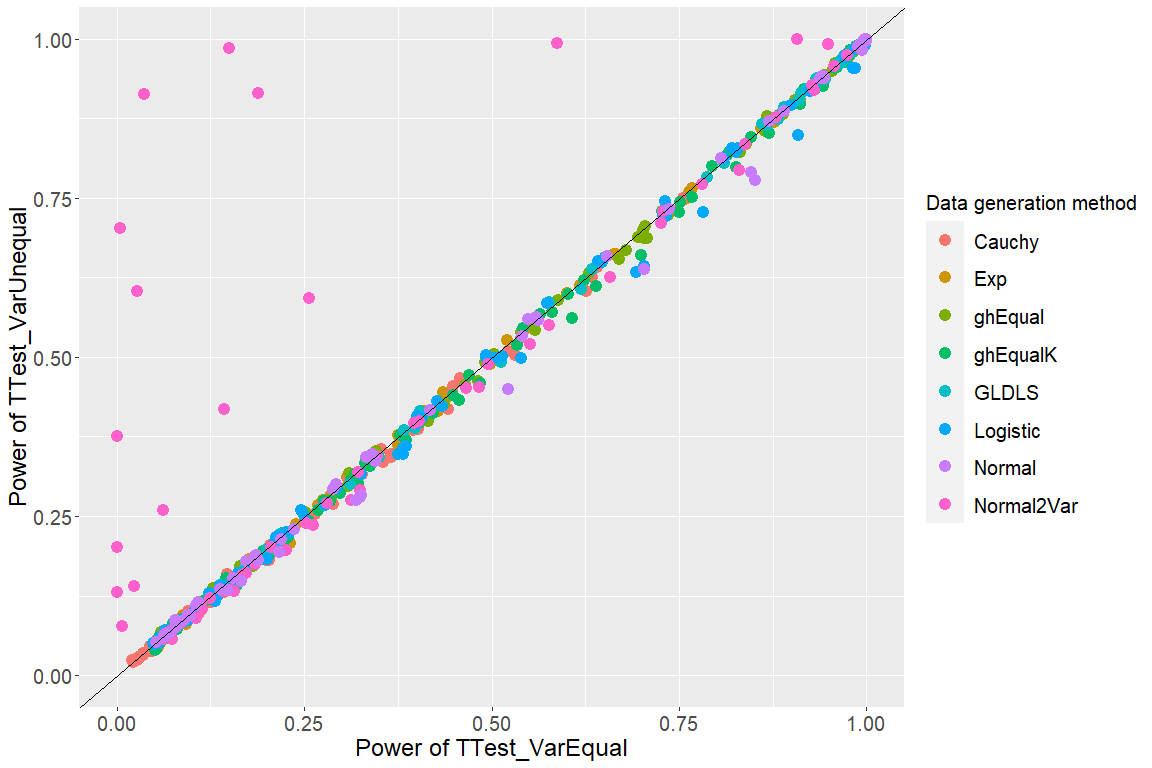
\includegraphics[width=0.5\linewidth]{report_files/figure-latex/figures-side-2} 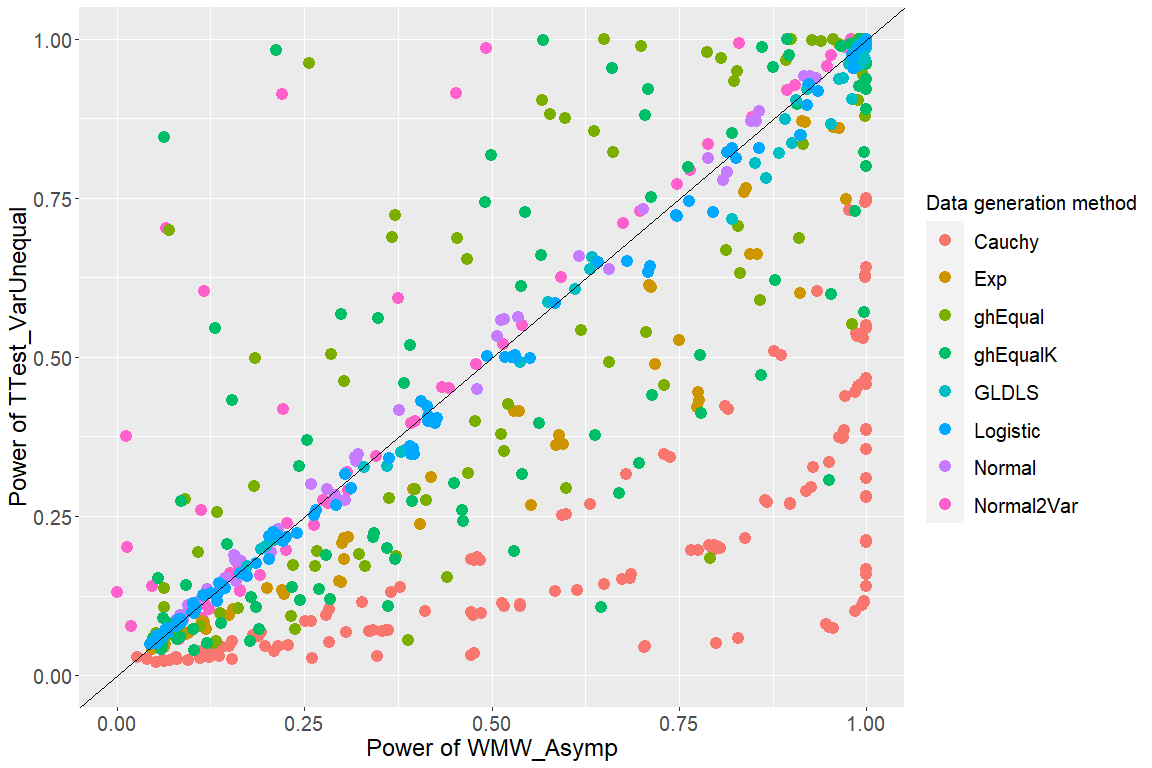
\includegraphics[width=0.5\linewidth]{report_files/figure-latex/figures-side-3} 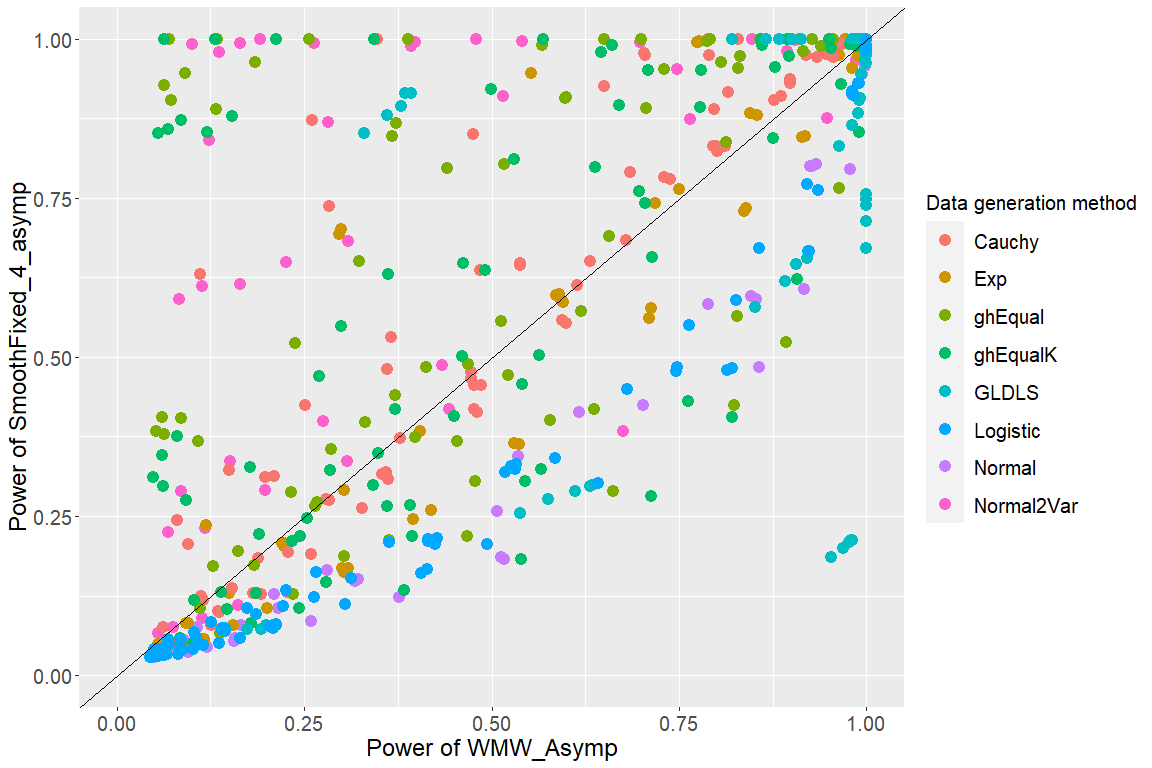
\includegraphics[width=0.5\linewidth]{report_files/figure-latex/figures-side-4} \caption{Power-Power plots for comparing two methods. Top left: Anderson-Darling versus Kolmogrov Smirnov test. Top right: Welch versus the two sample student-t test. Down left: Welch two sample test versus the Wilcoxon-Mann-Whitney test. Down Right: Two sample smooth test with fixed order 4 and Legendre polynomials versus the Wilcoxon-Mann-Whitney test.}\label{fig:figures-side}
\end{figure}

\hypertarget{conclusion}{%
\subsection{5. Conclusion}\label{conclusion}}

In terms of Type I error rate control the results has shown that the
Welch test and Yuen test, which is a derivative of the Welch test but
with trimmed means, do not perform well for skewed and heavy tailed
distributions in combination with unequal sample sizes. Moods test and
KS, have a conservative type I error rate control, especially for small
sample sizes. The methods that have a conservative type I error rate
have shown that they are also lacking in terms of power. AD has
performed well in most scenarios. The WMW test performed well in
scenarios with symmetrical distributions (with equal sample sizes), but
less in scenarios with opposite skewed distributions and heavy tailed
distributions.\\
In general, the methods perform well for the distributions and scenarios
they are developed for. The methods distinguish from each other in
scenarios that have small sample size and/or unequal balanced design, in
combination with skewed and heavy tailed distributions. Here, the more
robust methods such as AD, CVM perform better.

\end{document}
